\chapter{癫痫发作和癫痫} \label{chap:chap58}

直到最近,人类大脑皮层(大脑中与知觉、运动和认知功能有关的区域)的功能和组织一直困扰着临床医生和神经科学家。
过去,对脑功能的分析主要依赖于对中风或外伤引起的脑损伤和细胞丢失导致的脑功能丧失的观察。
这些自然实验提供了许多早期证据,表明不同的大脑区域具有特定功能,或者正如美国著名神经学家 C. Miller Fisher 所说,“我们了解大脑‘中风’。”
对癫痫发作和癫痫患者的观察已经 在脑功能研究中同样重要,因为这些神经活动过度障碍的行为后果告诉临床医生激活如何影响它们起源的大脑区域。


由异常、过度的神经元活动引起的脑功能暂时性破坏称为癫痫发作,而反复发作的慢性病称为癫痫。
几个世纪以来,对癫痫发作的神经学起源的理解因与癫痫发作相关的戏剧性的、有时甚至是怪异的行为而感到困惑。
癫痫的慢性病症广泛与邪灵附身有关,但癫痫发作也被认为是神谕、先见之明或特殊创造力的标志。


希波克拉底时代(大约公元前 400 年)的希腊人意识到大脑一侧的头部受伤可能会导致身体另一侧的癫痫发作。
在那些早期,癫痫的诊断可能比当代的定义要广泛得多。
发作性无意识的其他原因,例如晕厥以及大规模歇斯底里和心因性癫痫发作,几乎可以肯定归因于癫痫。
此外,历史著作通常描述涉及两个大脑半球的全身性抽搐发作;
因此,涉及大脑非常有限区域的癫痫发作很可能被误诊或根本没有被诊断出来。
即使在今天,医生也很难区分发作性意识丧失和各种类型的癫痫发作。
然而,随着我们治疗甚至治愈癫痫的能力不断提高,这些诊断区别变得越来越重要。


癫痫的早期神经生物学分析始于 1860 年代约翰·休林斯·杰克逊 (John Hughlings Jackson) 在伦敦的工作。
杰克逊意识到,癫痫发作不一定涉及意识丧失,但可能与手臂抽搐等局部症状有关。
他的观察是对我们现在所说的部分(或局灶性)癫痫发作的首次正式认识。
杰克逊还观察到患者的癫痫发作以局灶性神经系统症状开始,然后通过以有序的方式稳定地累及邻近区域(所谓的杰克逊式进行曲)发展为伴随意识丧失的抽搐。
早在使用电生理技术建立功能组织之前(第 ~\ref{chap:chap4}~章),他的观察就产生了运动小人的概念(代表身体组织的解剖图或皮层表面的“接线图”)。


另一个预示着现代疗法的开创性发展是 1886 年英国神经外科医生维克多·霍斯利 (Victor Horsley) 首次对癫痫进行手术治疗。
霍斯利切除了与凹陷性颅骨骨折相邻的大脑皮层,并治愈了一名局灶性运动性癫痫发作的患者。
相 癫痫常规手术治疗的诞生可以追溯到 20 世纪 50 年代初,当时蒙特利尔的 Wilder Penfield 和 Herbert Jasper 在移除癫痫病灶之前刺激皮质并精确定位运动和感觉图。
与任何慢性疾病一样,癫痫发作的生理特征并不是癫痫患者护理和管理的唯一考虑因素。
社会心理因素也极为重要。 癫痫的诊断会影响日常生活的方方面面,包括教育机会、驾驶和就业。
尽管对癫痫患者施加的许多社会限制是适当的——大多数人会同意癫痫患者不应该成为商业飞行员——癫痫的诊断可能会对教育机会和就业产生不适当的负面影响。
为了改善这种情况,医生有责任就癫痫及其主要合并症(包括认知问题和抑郁症)的基础科学知识对自己和公众进行教育。



\section{癫痫发作和癫痫的分类对于发病机制和治疗很重要}

并非所有癫痫发作都是一样的。
因此,癫痫发作的发病机制和分类必须考虑到每个患者的临床特征以及获得性和遗传因素。
癫痫发作和反复发作的慢性病症(癫痫)很常见。
根据美国的流行病学研究,所有活到 80 岁的人中有 1\% 到 3\% 会被诊断出患有癫痫症。
发病率最高的是幼儿和老年人。


在许多方面,癫痫发作代表一种原型神经系统疾病,因为症状包括“阳性”和“阴性”感觉或运动表现。
癫痫发作期间可能出现的阳性体征示例包括对闪光的感知或手臂的抽搐。
阴性体征反映正常大脑功能受损,例如意识和认知意识受损,甚至短暂性失明、言语停止或瘫痪。
这些例子强调了癫痫发作的一般特征:
体征和症状取决于受影响的大脑区域的位置和范围。
最后,癫痫发作的表现部分是由具有正常细胞和网络特性的周围组织触发的同步活动引起的。
后一种活动对于癫痫发作超出其原始边界的传播尤为重要——癫痫发作完全可以劫持大脑的正常功能。



\subsection{癫痫发作是大脑功能的暂时性破坏}

癫痫发作在临床上根据发作时间分为局灶性或全身性两类(表 58-1)。
这种分类在概念上很简单,但由于多年来使用了多个术语来指代相同的情况,二元性质可能已经模糊不清。
尽管如此,这种癫痫发作分类已被证明对临床医生非常有用,并且抗惊厥药物针对一种或另一种类型。


局灶性发作(也称为部分性发作)起源于一小群神经元(癫痫病灶),因此症状取决于病灶在大脑中的位置。
局灶性癫痫发作既可以在没有意识改变的情况下发生(通常称为简单部分发作),也可以在意识改变的情况下发生(通常称为复杂部分发作)。
典型的局灶性癫痫发作可能从右手抽搐开始,然后发展为整个右臂的阵挛性运动(即抽搐)。
如果局灶性癫痫发作进一步发展,患者可能会失去知觉、倒地、四肢僵硬地伸展(强直期),然后四肢出现痉挛性抽搐(阵挛期)。


局灶性癫痫发作之前可能会出现称为先兆的明显症状。
常见的先兆包括无端的、通常是生动的感觉,例如恐惧感、腹部上升的感觉,甚至是特定的气味。
小说家陀思妥耶夫斯基将他的光环描述为“一种感觉……如此强烈和甜蜜,以至于为了这种幸福的几秒钟,我愿意付出我生命中十年或更长时间,甚至可能是我的整个生命。” 
先兆是癫痫病灶中电活动的产物,因此代表了最早的癫痫发作表现。
癫痫发作后但在患者恢复其正常神经功能水平之前的时间称为发作后期。


全身性发作构成第二个主要类别。
它们开始时没有先兆或局灶性发作,并且从一开始就涉及两个半球。
因此,它们有时被称为原发性全身性发作,以避免与局灶性发作后继发性全身性发作混淆。
根据癫痫发作是否与强直-阵挛运动相关,全身性发作可进一步分为运动(惊厥)或非运动类型。


原型非运动性全身性发作是儿童典型的失神发作(以前称为小发作)。
这些癫痫发作突然开始,通常持续不到 10 秒,与凝视和所有运动活动突然停止有关,并导致意识丧失但不会失去姿势。
患者似乎处于恍惚状态,但发作非常短暂,不经意的观察者可能会错过。
与局灶性癫痫发作不同,癫痫发作前没有先兆或癫痫发作后(发作后时期)没有意识模糊。
患者可能表现出轻微的运动表现,例如眨眼,但不会跌倒或有强直阵挛运动。
典型的失神发作在脑电图上具有非常独特的电气特征,称为棘波模式。


一些全身性癫痫发作仅涉及异常(肌阵挛、阵挛或强直)运动或运动张力突然丧失(失张力)。
最常见的全身性癫痫发作的运动类型是强直阵挛(以前称为大发作)发作。
这种癫痫发作突然开始,通常伴有咕噜声或哭声,因为膈肌和胸廓的强直收缩迫使呼气。
在强直期,患者可能会以僵硬的姿势倒地,咬紧牙关,大小便失控,脸色发青(紫绀)。
强直阶段通常持续 30 秒,然后演变成持续 1 至 2 分钟的四肢阵挛性抽搐。
该活动期之后是发作后期,在此期间患者昏昏欲睡、迷失方向,并可能抱怨头痛和肌肉酸痛。


全身性强直阵挛性癫痫发作可能难以从纯粹的临床基础上与具有短暂先兆的局灶性癫痫发作区分开来,后者会迅速发展为全身性强直阵挛性癫痫发作。
这种区别不是学术性的,因为它对于查明根本原因和选择适当的治疗方法至关重要。
然而,一些癫痫发作由于起病时间不确定而难以分类。



\subsection{癫痫是一种反复发作的慢性疾病}

反复发作是诊断癫痫的最低标准。
经常被引用的临床规则“单次癫痫发作不会造成癫痫”强调了这一点,甚至因酒精戒断等刺激而反复发作也不算癫痫。
在表 58-1 中的癫痫发作分类方案中忽略了导致反复发作临床模式的各种因素——癫痫发作的潜在病因、发作年龄或家族史。
癫痫的分类主要基于临床观察而不是对疾病的精确细胞、分子或遗传理解。
影响癫痫发作类型和严重程度的因素通常可以识别为体征和症状的模式,称为癫痫综合征。
这些因素包括癫痫发作的年龄、癫痫发作是否遗传以及脑电图上的某些模式。
对这些综合征的认识在最近发现单基因突变是癫痫发作的原因中发挥了作用。


癫痫分类的主要变量是是否可以识别局灶性脑异常(与局限性相关的癫痫与全身性癫痫)以及是否存在可识别的原因(症状性)(未知,通常称为特发性)。
绝大多数成人发作的癫痫被归类为症状性定位相关性癫痫。
此类别包括外伤、中风、肿瘤和感染等原因。
很多人患有成年发作的癫痫,但没有明确的病因。


不幸的是,尽管这种分类方案很有用,但许多癫痫综合征并不完全适合。
人们期望(并希望)这种分类将得到极大的改进,因为标准包括潜在的病因而不仅仅是临床表型。



\section{脑电图代表皮层神经元的集体活动}

因为神经元是可兴奋的细胞,所以癫痫发作直接或间接由单个神经元或神经元群的兴奋性变化引起也就不足为奇了。
这种观点主导了癫痫发作的早期实验研究。
为研究此类效应,可以使用细胞内或细胞外电极对大脑活动进行电记录。
细胞外电极感应附近神经元的动作电位,并可以检测称为场电位的细胞群的同步活动。


在细胞外记录的缓慢时间分辨率(数百毫秒到几秒)下,场电位可以表现为称为尖峰的单个瞬态变化。
这些尖峰反映了许多神经元中的动作电位,不应与单个神经元记录中的尖峰混淆,后者是仅持续 1 或 2 毫秒的单个动作电位。
因此,脑电图代表一组场电位,由头皮表面的多个电极记录(图~\ref{fig:58_1})。


\begin{figure}[htbp]
	\centering
	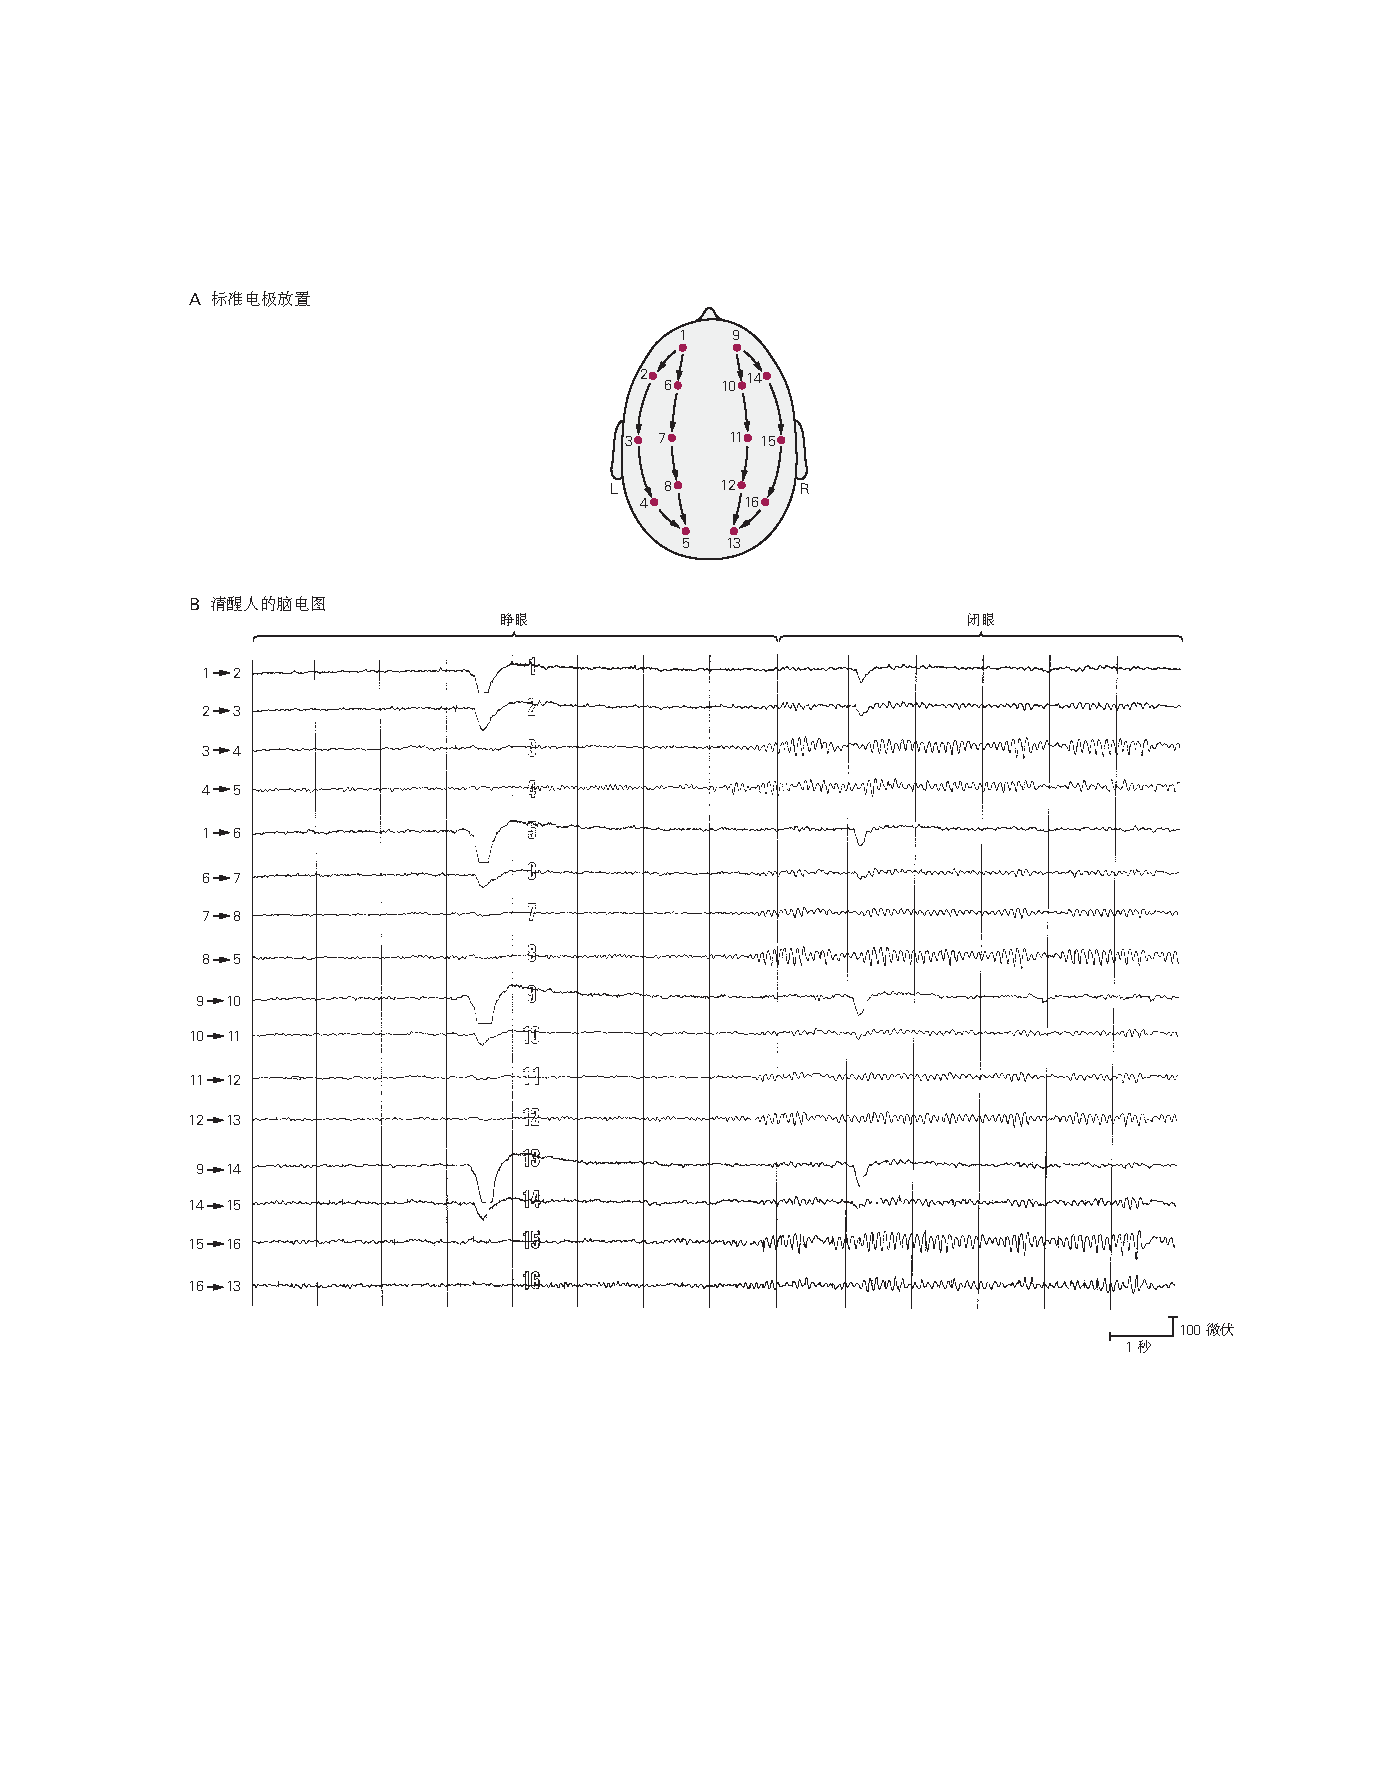
\includegraphics[width=0.95\linewidth]{chap58/fig_58_1}
	\caption{清醒人类受试者的正常脑电图 (EEG)。 A. 头皮表面的一组标准电极放置(或蒙太奇)。每个位置的电响应反映了两个电极之间的活动。B. 在录音开始时,脑电图显示头皮表面存在低电压活动(~20 μV)。 垂直线以 1 秒为间隔放置。 在最初的 8 秒内,受试者睁着眼睛静静地休息,然后要求受试者闭上眼睛。闭眼时,枕骨区域(位点 3、4、8、12、15 和 16)会出现更大幅度的活动 (8–10 Hz)。这是放松、清醒状态的正常阿尔法节律特征。眨眼时 3.5 秒和闭眼时 9 秒时会出现缓慢的大振幅伪影。}
	\label{fig:58_1}
\end{figure}


由于电活动起源于下层脑组织中的神经元,因此表面电极记录的波形取决于电源相对于电极的方向和距离。
EEG 信号不可避免地会因组织和骨骼的介入层引起的滤波和衰减而失真,这些组织和骨骼的作用与回路中的电阻器和电容器相同。
因此,EEG 信号的振幅(以微伏为单位)远小于单个神经元的电压变化(毫伏)。
单个细胞中的高频活动,例如动作电位,被 EEG 信号滤除,这主要反映了细胞膜上较慢的电压变化,例如突触电位。


尽管 EEG 信号是对由许多神经元的总电活动引起的细胞外电流的测量,但并非所有细胞对 EEG 的贡献都相同。
表面脑电图主要反映了靠近头皮上每组脑电图电极的皮层神经元的活动。
因此,皮层回底部、大叶内侧壁、海马体、丘脑或脑干等深层结构对表面脑电图没有直接贡献。
方框~\ref{box:58_1}~中讨论了单个神经细胞对 EEG 的贡献。


\begin{proposition}[单个神经元对脑电图的贡献] \label{box:58_1}
	
	\quad \quad 单个神经元的活动对脑电图(EEG)的贡献可以通过检查简化的皮层电路和一些基本的电学原理来理解。
	锥体神经元是大脑皮层的主要投射神经元。
	这些细胞的顶端树突垂直于细胞表面,接受各种突触输入。
	因此,锥体细胞的突触活动是脑电活动的主要来源。
	
	了理解单个神经元对EEG的贡献,考虑皮层锥体神经元顶端树突上的兴奋性突触后电位产生的电荷流(图58-2)。
	离子电流在兴奋性突触后电位产生的位置进入枝晶,产生通常所说的电流汇。
	然后,它必须沿着树枝状结构向下流动,然后在其他位置穿过膜,形成电流源,从而完成一个循环。
	
	突触电流产生的电压信号大致由欧姆定律预测(V=IR,其中V是电压,I是电流,R是电阻)。
	因为膜电阻(Rm)远大于构成细胞外介质的盐溶液的电阻(Re),所以用细胞内电极(Vm)在膜上记录的电压也大于位于电流汇附近的细胞外电极(Ve)处的电压。
	
	在EPSP的产生位点,细胞外电极检测到由于电荷从电极流入细胞质而引起的电压变化,作为负电压偏转。
	然而,电流源附近的细胞外电极记录了相反极性的信号(比较图58-2中的电极1和3)。
	如果兴奋性突触后电位产生的部位在顶端树突的基底段,情况就会逆转。
	
	在大脑皮层中,来自对侧半球的兴奋性轴突主要终止于II层和III层的树突,而丘脑皮层轴突终止于IV层(图58-2)。
	因此,即使电事件(膜去极化)相同,由表面EEG电极测量的活动对于这两个输入将具有相反的极性。
	
	类似地,皮层突触事件的起源或极性不能仅从表面脑电图记录中明确确定。
	浅层的EPSP和深层的抑制性突触后电位(IPSP)均表现为向上(负)电位,而深层的EPSP与浅层的IPSP具有向下(正)电位(图58-3)。
	
\end{proposition}


表面脑电图显示活动模式——以电活动的频率和幅度为特征——与睡眠和觉醒的不同阶段(第 ~\ref{chap:chap44}~章)以及一些病理生理过程(如癫痫发作)相关。
正常人脑电图显示 1 到 30 Hz 范围内的活动,振幅在 20 到 100 μV 范围内。
观察到的频率被分为几组:alpha (8–13 Hz)、beta (13–30 Hz)、delta (0.5–4 Hz) 和 theta (4–7 Hz)。


中等振幅的 α 波是典型的放松清醒状态,在顶叶和枕叶部位最为突出。
在激烈的心理活动中,较低振幅的 β 波在额叶区域和其他区域更为突出。
通过要求他们睁开眼睛来警告放松的受试者会导致所谓的 EEG 去同步化,同时 alpha 活动减少和 beta 活动增加(图~\ref{fig:58_1}B)。
Theta 和 delta 波在困倦和早期慢波睡眠期间是正常的;
如果它们在清醒时出现,则表明大脑功能障碍。


随着神经元整体变得同步,当受试者放松或变得昏昏欲睡时,总电流变得更大,并且可以看作是基线活动的突然变化。
这种“阵发性”活动可能是正常的,例如,在睡眠期间发生的高振幅活动(1-2 秒,7-15 赫兹)(睡眠纺锤波)。
然而,尖波或 EEG 尖峰信号也可以为癫痫患者的癫痫病灶位置提供线索(图~\ref{fig:58_4})。
新的记录和分析方法,如脑电图的频谱分析,越来越多地被用于检测癫痫病灶内的异常同步区(快速波纹)。


\begin{figure}[htbp]
	\centering
	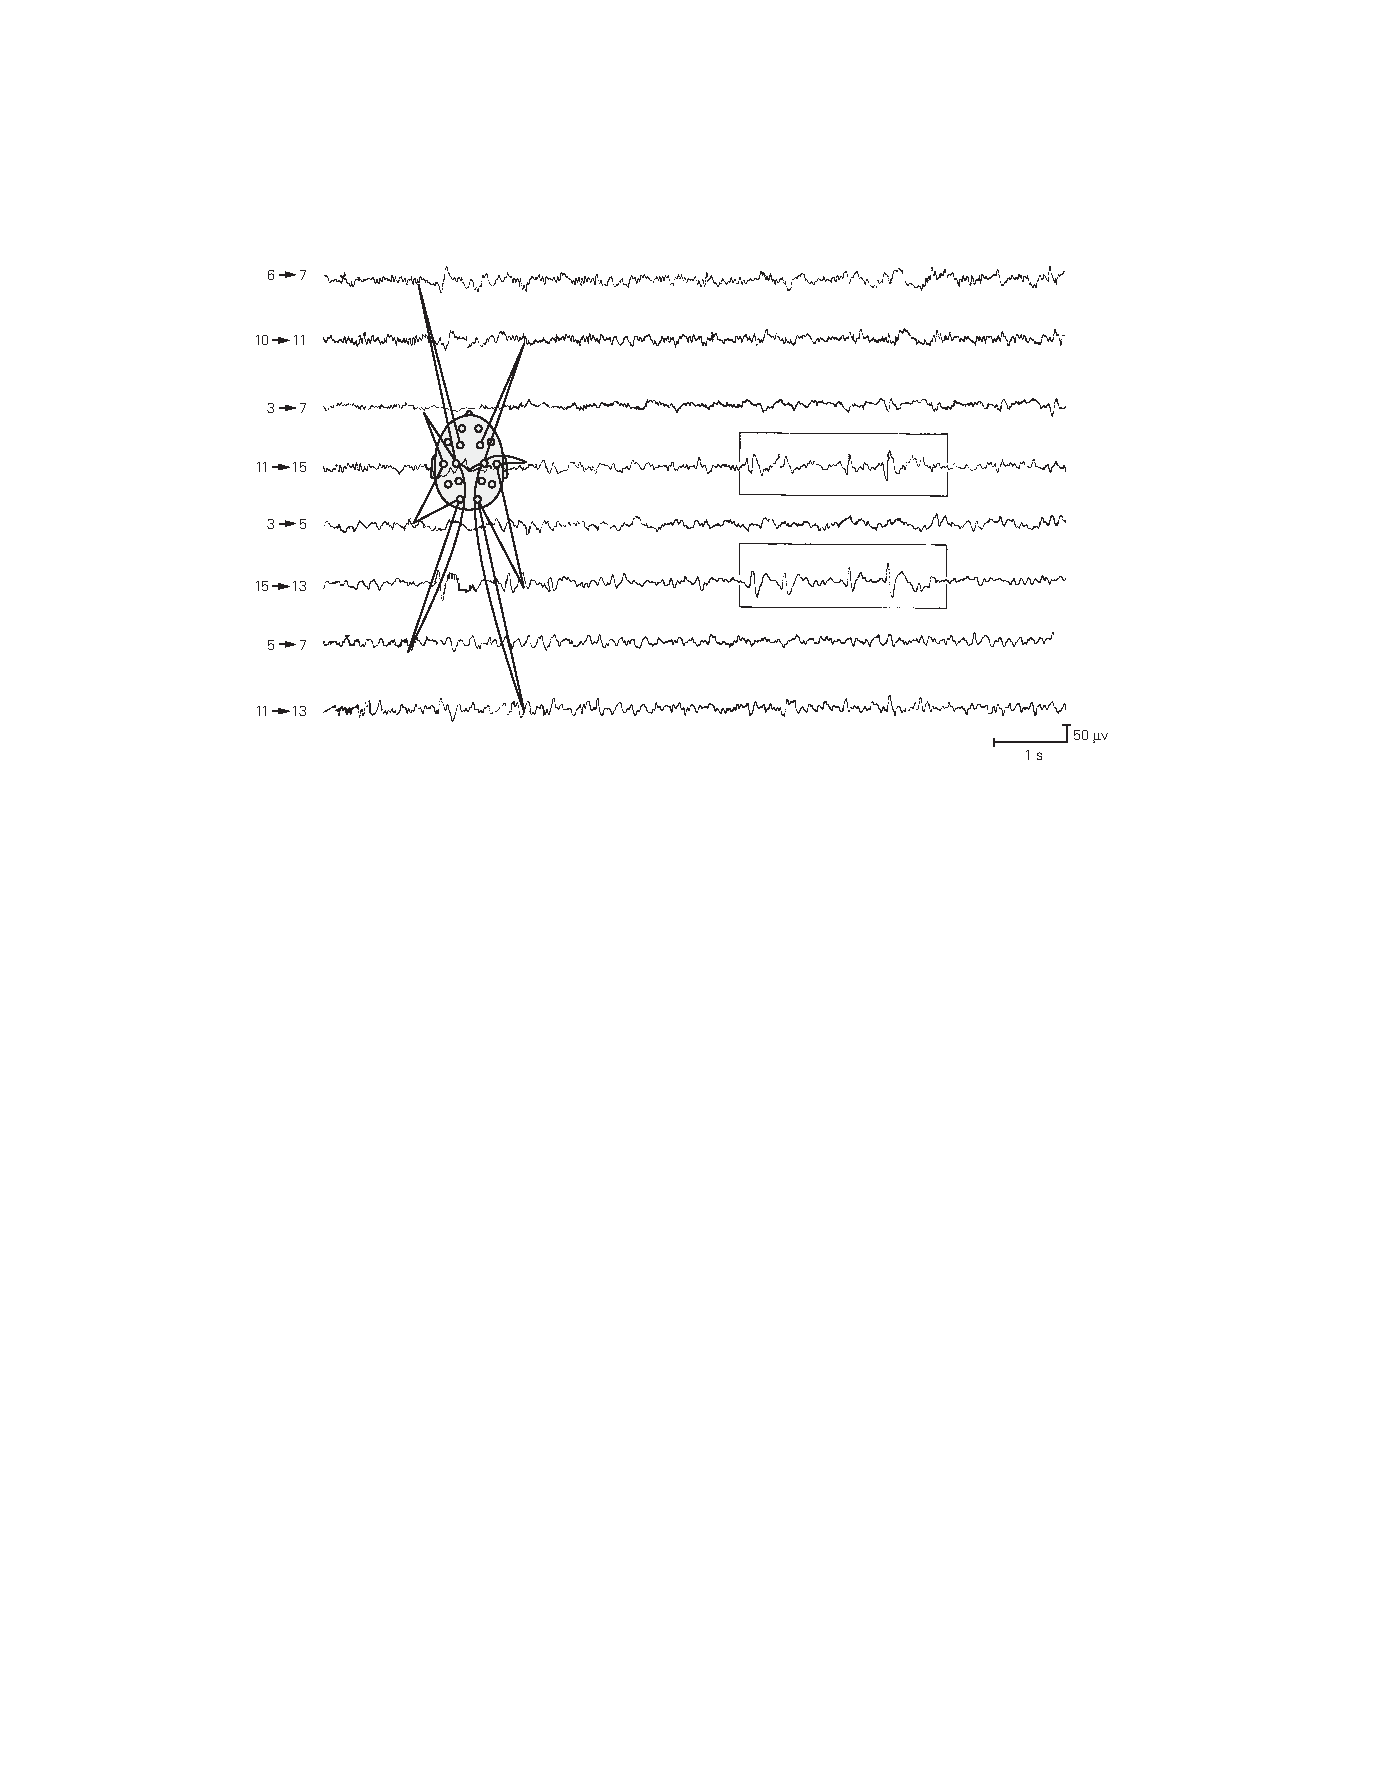
\includegraphics[width=0.8\linewidth]{chap58/fig_58_4}
	\caption{脑电图 (EEG) 可以提供癫痫病灶位置的线索。每条迹线代表电极图中所示的头皮电极对之间的电活动。例如,电极对 11–15 和 15–13 测量右侧颞区的活动。癫痫患者的脑电图活动显示右侧颞区的电极出现尖波(记录在盒子中)。这种阵发性活动突然出现并破坏了正常的背景 EEG 模式。局灶性异常可能表明该患者的癫痫病灶位于右颞叶。因为患者在记录期间没有临床发作,所以这些是发作间期尖峰(见图~\ref{fig:58_7})。(经许可改编自 Lothman 和 Collins 1990。)}
	\label{fig:58_4}
\end{figure}



\section{局灶性癫痫发作起源于一小群神经元}

尽管临床上定义的癫痫发作多种多样,但通过比较局灶性癫痫发作与全身性癫痫发作的电图模式,可以在很大程度上理解对癫痫发作活动产生的重要见解。


局灶性癫痫发作的定义特征是异常电活动源自癫痫病灶。
癫痫病灶被认为只不过是一小群神经元,可能有 1 千个左右,它们具有增强的兴奋性和偶尔将这种活动传播到邻近区域的能力,从而引起癫痫发作。
增强的兴奋性(癫痫样活动)可能由许多不同的因素引起,例如细胞特性改变、神经胶质功能障碍或由局部疤痕、血凝块或肿瘤引起的突触连接改变。
局灶性发作的发展可任意分为四个阶段:(1) 发作间期,然后是 (2) 发作病灶内同步活动,(3) 发作扩散,最后,(4) 继发性泛化 . 阶段 2 到 4 代表癫痫发作的发作阶段。
每个阶段都有不同的因素。


我们关于癫痫发作期间电事件的大部分知识来自对局灶性癫痫发作动物模型的研究。
通过局灶性电刺激或通过急性注射惊厥剂在动物中诱发癫痫发作。
这种方法以及来自这些动物模型的组织的体外研究提供了对癫痫发作期间以及发作间期发作期间病灶内电事件的良好理解。



\subsection{癫痫病灶中的神经元有异常的爆发活动}

单个神经元或一组神经元的电活动如何导致局灶性癫痫发作?
癫痫病灶内的每个神经元都有刻板和同步的电反应,阵发性去极化偏移,去极化是突然的、大的 (20-40 mV) 和持久的 (50-200 毫秒),并触发一系列动作电位达到顶峰。
阵发性去极化偏移之后是后超极化(图~\ref{fig:58_5}A)。


\begin{figure}[htbp]
	\centering
	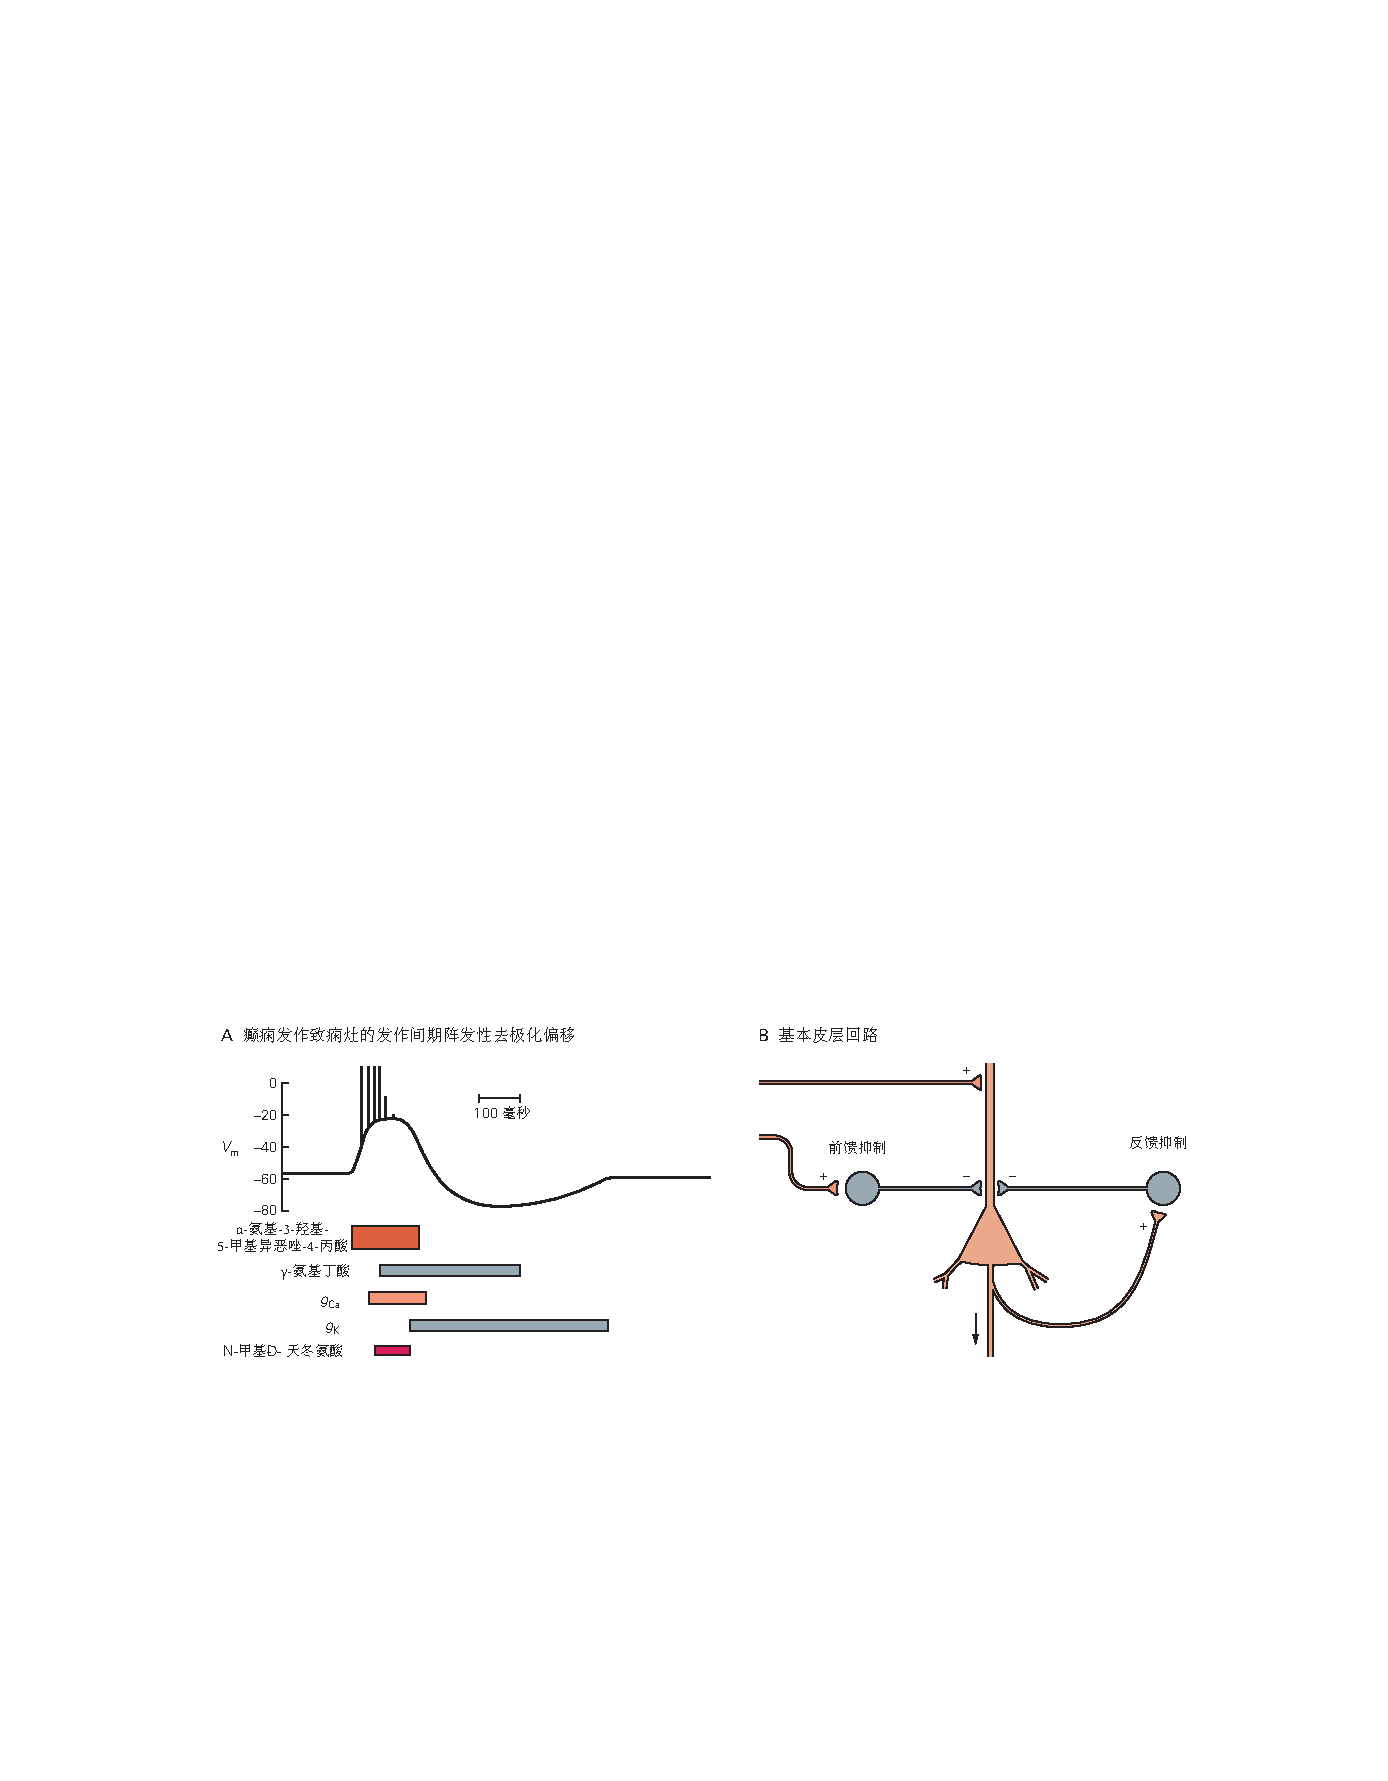
\includegraphics[width=0.9\linewidth]{chap58/fig_58_5}
	\caption{癫痫病灶中神经元阵发性去极化转变的电导。A. 阵发性去极化偏移 (PDS) 在很大程度上取决于 α-amino-3-hydroxy-5-methyl-4-isoxazolepropionic acid (AMPA)- 和\textit{N-甲基-D-天冬氨酸}-type glutamate receptor-channels 其有效性通过电压门控 Ca2+ 通道 (gCa) 的打开而增强。 去极化后,细胞通过激活 γ-氨基丁酸 (GABA) 受体(离子型 GABAA 和代谢型 GABAB)以及电压门控和钙激活 K+ 通道 (gK) 而超极化。 (经许可改编自 Lothman 1993a。)B. 反复出现的轴突分支激活抑制性神经元并引起锥体神经元的反馈抑制。 外在兴奋性输入也可以激活前馈抑制。PDS 代表癫痫病灶中的过度兴奋,而抑制回路构成环绕抑制的基础,对于将发作间期活动限制在癫痫病灶中很重要。}
	\label{fig:58_5}
\end{figure}


阵发性去极化偏移和后超极化由神经元的内在膜特性(例如,电压门控 Na+、K+ 和 Ca2+ 通道)和来自兴奋性和抑制性神经元(分别主要是谷氨酸能和 GABA 能)的突触输入形成。
去极化阶段主要是由 α-amino-3-hydroxy-5-methyl-4-isoxazolepropionic acid (AMPA)- 和\textit{N-甲基-D-天冬氨酸}- 型谷氨酸受体通道的激活引起的(图~\ref{fig:58_5}A),以及电压门控 Na+ 和 Ca2+ 通道。
\textit{N-甲基-D-天冬氨酸}型受体通道在增强兴奋性方面特别有效,因为去极化解除了通道的 Mg2+ 阻塞。
清除阻塞会增加通过通道的电流,从而增强去极化并允许额外的 Ca2+ 进入神经元(第~\ref{chap:chap13}~章)。


皮质锥体神经元对兴奋性输入的正常反应包括兴奋性突触后电位,然后是抑制性突触后电位 (IPSP)(图 ~\ref{fig:58_5}B)。
因此,阵发性去极化偏移可以被视为这些去极化和超极化突触成分的大量增强。
后超极化由电压依赖性和 Ca2+ 依赖性 K+ 通道以及 γ-氨基丁酸 (GABA) 介导的 Cl– 电导(离子型 GABAA 受体)和 K+ 电导(代谢型 GABAB 受体)产生(图~\ref{fig:58_5}A) )。
Ca2+ 通过电压依赖性 Ca2+ 通道和\textit{N-甲基-D-天冬氨酸}型受体通道流入会触发钙激活通道的打开,尤其是 K+ 通道。
后超极化限制了阵发性去极化偏移的持续时间,其逐渐消失是局灶性癫痫发作的最重要因素,如后所述。


因此,许多惊厥药通过增强兴奋或阻断抑制作用就不足为奇了。
相反,抗惊厥药可以通过阻断兴奋或增强抑制作用。 例如,苯二氮卓类地西泮 (Valium) 和劳拉西泮 (Ativan) 可增强 GABAA 介导的抑制作用,并用于紧急治疗长时间重复性癫痫发作。
抗惊厥药苯妥英 (Dilantin) 和卡马西平 (Tegretol) 以及其他几种药物可减少作为动作电位基础的电压门控 Na+ 通道的开放。
Na+ 通道的分子模型表明,当通道处于开放或激活状态时,这些药物更有效。
因此,恰如其分地,这些药物阻断 Na+ 通道的能力因与癫痫发作相关的重复活动而增强;
也就是说,影响最大的是那些最需要沉默的神经元。



\subsection{环绕抑制的崩溃导致同步}

只要异常电活动仅限于一小部分神经元,就没有临床表现。
癫痫病灶中神经元的同步不仅取决于每个细胞的内在特性,还取决于神经元之间连接的数量和强度。
在发作间期,异常活动通过周围组织的抑制作用被限制在癫痫病灶内。


这种“抑制性环绕”最初由 David Prince 描述,特别依赖于 GABA 能抑制性中间神经元的前馈和反馈抑制(图~\ref{fig:58_6}A)。
尽管大脑皮层中的抑制回路通常用简单的图表表示(图 ~\ref{fig:58_6}B),但皮层抑制神经元的形态和连接性实际上相当复杂,并且是使用许多新方法(例如细胞类型特异性病毒标记)继续研究的主题 和光遗传学刺激。


\begin{figure}[htbp]
	\centering
	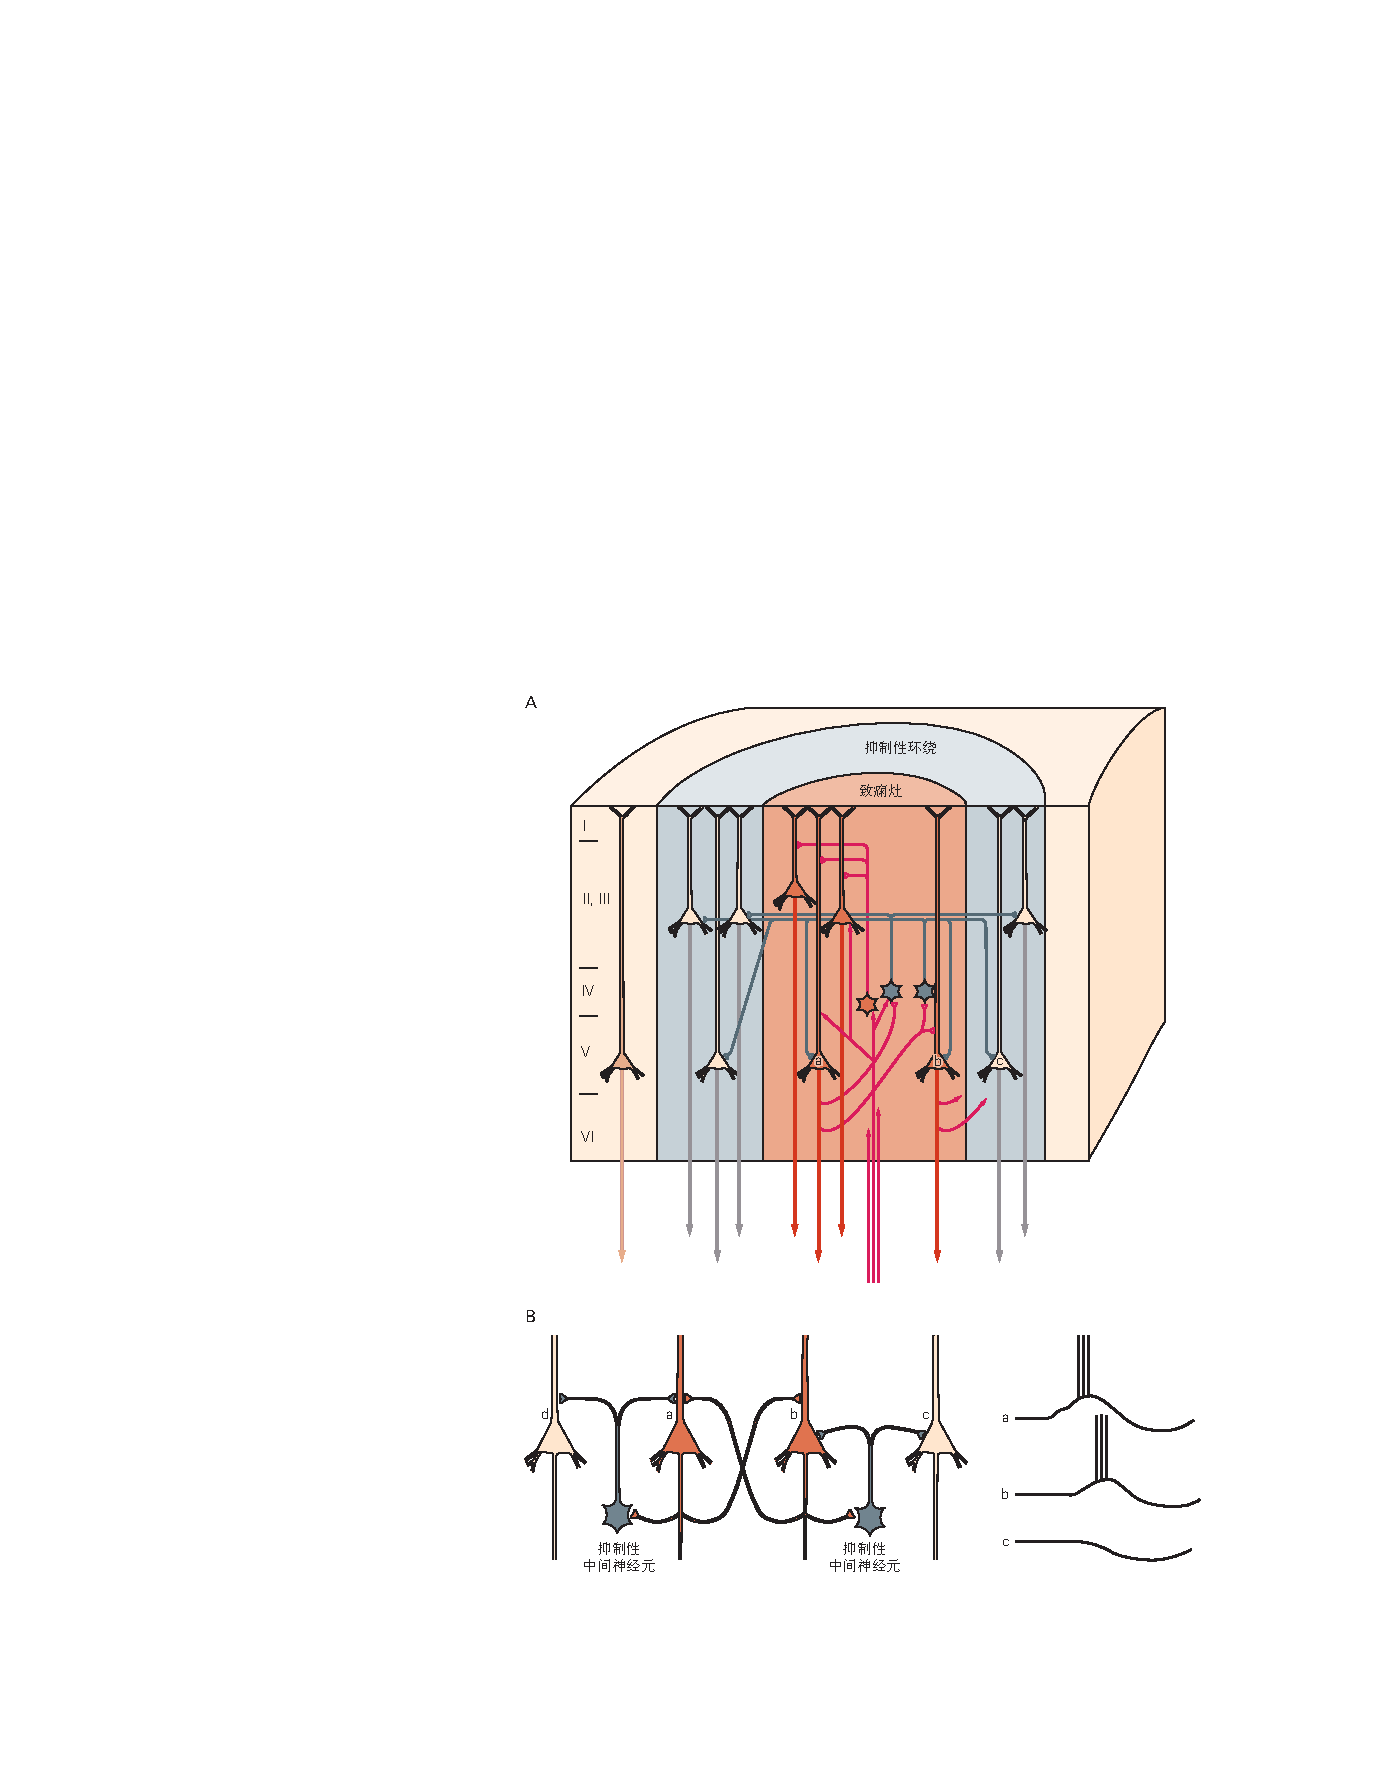
\includegraphics[width=0.7\linewidth]{chap58/fig_58_6}
	\caption{癫痫病灶的空间和时间组织取决于病灶中神经元的兴奋和抑制之间的相互作用。A. 锥体细胞 a 显示癫痫病灶中神经元的典型电学特性(参见 B 部分)。细胞 a 中的兴奋会激活另一个锥体细胞 (b),当许多此类细胞同时放电时,脑电图上就会记录到尖峰信号。然而,细胞 a 也激活 γ-氨基丁酸 (GABA)-能抑制中间神经元(灰色)。这些中间神经元可以通过反馈抑制降低细胞 a 和 b 的活动,从而在时间上限制癫痫病灶,并防止病灶外的细胞放电,此处由细胞 c 表示。 后一种现象会产生一种抑制性环境,在发作间期抑制对癫痫病灶的过度兴奋。当外在或内在因素改变这种兴奋和抑制的平衡时,抑制性环境开始瓦解,癫痫发作活动扩散,导致癫痫发作。 (经许可改编自 Lothman 和 Collins 1990。)B. A 部分所示的细胞 a、b 和 c 的突触连接和活动模式。细胞 a 和 b(在癫痫病灶内)经历阵发性去极化转变, 而细胞 c(在抑制性周围)由于来自 GABAergic 抑制性中间神经元的输入而超极化。}
	\label{fig:58_6}
\end{figure}


在局灶性发作的发展过程中,回路中的兴奋克服了抑制性环绕,原灶神经元的后超极化逐渐消失。
结果,产生了几乎连续的高频动作电位序列,癫痫发作开始扩散到原始病灶之外(图~\ref{fig:58_7})。


\begin{figure}[htbp]
	\centering
	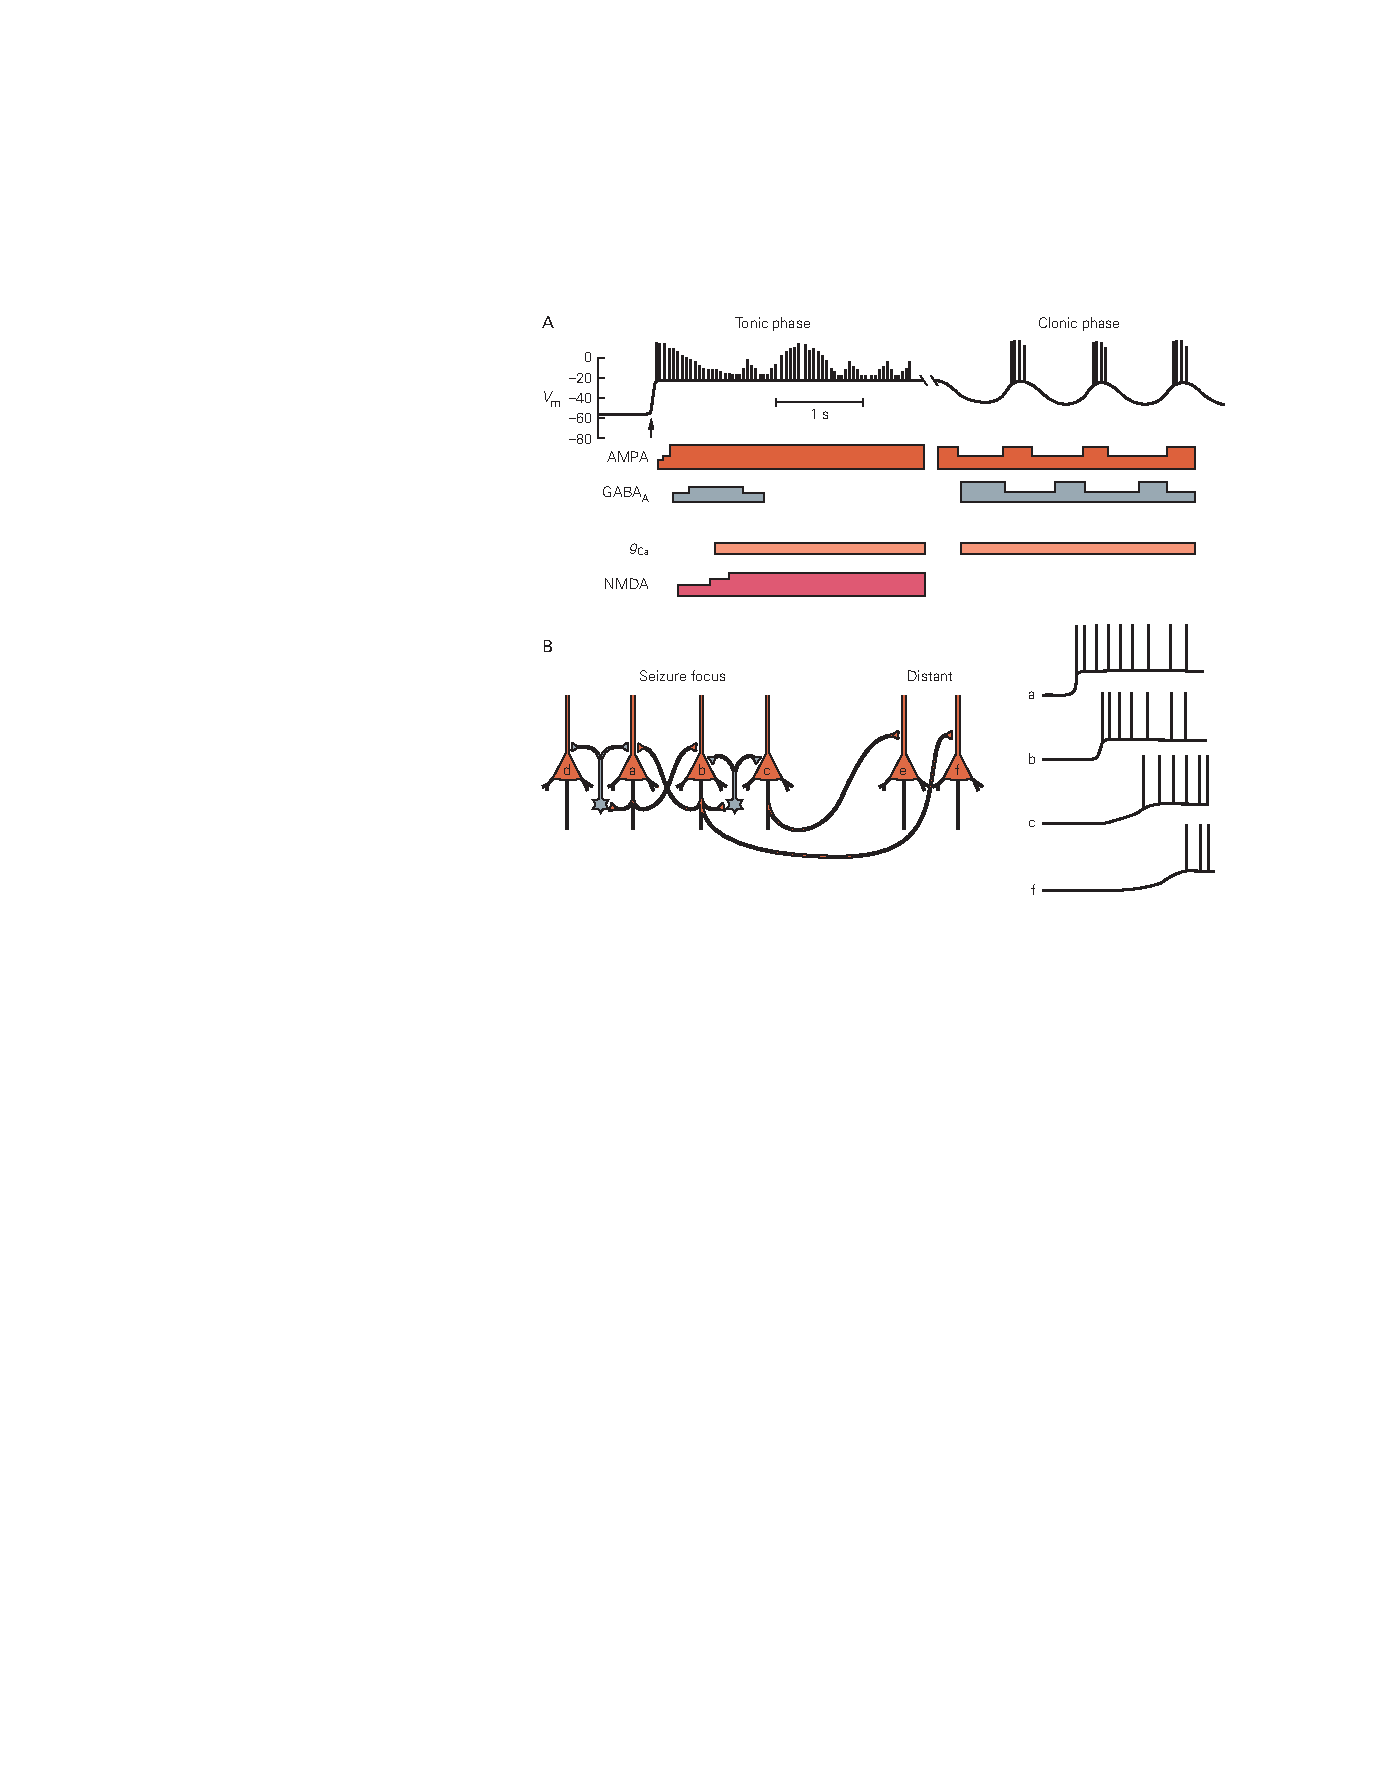
\includegraphics[width=0.7\linewidth]{chap58/fig_58_7}
	\caption{局灶性发作开始于后超极化和周围抑制的丧失。(经许可改编自 Lothman 1993a。)A. 随着发作的开始(箭头),发作灶中的神经元去极化,就像阵发性去极化转变的第一阶段一样。然而,与发作间期不同的是,去极化持续数秒或数分钟。γ-氨基丁酸 (GABA) 介导的抑制作用失败,而 α-氨基-3-羟基- 5-甲基-4-异恶唑丙酸 (AMPA)- 和\textit{N-甲基-D-天冬氨酸}- 的兴奋性活性 型谷氨酸受体功能增强。这种活动对应于继发性全身性强直阵挛发作的强直期。随着 GABA 介导的抑制逐渐恢复,癫痫病灶中的神经元进入与阵挛期相对应的振荡期。B. 随着周围抑制的瓦解,癫痫病灶中的神经元同步兴奋,并向远处的神经元发送一系列动作电位,从而从病灶传播异常活动。将细胞 a 到 c 中的这种活动模式与发作间期的活动模式进行比较(图 58-6B)。}
	\label{fig:58_7}
\end{figure}


局灶性癫痫发作扩散的一个重要因素似乎是锥体神经元的强烈放电导致抑制性 GABA 能中间神经元的突触传递相对减少,尽管中间神经元仍然存活。
这种减少是由 GABA 释放的突触前变化还是 GABA 受体的突触后变化引起的尚不清楚,并且在所有情况下可能都不相同。
随着时间的推移,可能导致抑制性环绕丧失的其他因素包括树突形态的变化、受体或通道的密度,或由细胞外 K+ 离子积累引起的 EK 的去极化转变。
长时间放电还会将动作电位传输到大脑中的远端位置,这反过来可能会触发神经元中的动作电位序列,这些动作电位序列会投射回癫痫病灶中的神经元(反向传播)。
在这方面,新皮层和丘脑之间的相互联系可能特别重要。


尽管我们了解这些机制,但我们仍然不知道是什么原因导致癫痫发作在任何特定时刻发生。
无法预测癫痫发作的时间可能是癫痫最令人虚弱的方面。
方框~\ref{box:58_2}~中讨论了解决这一难题的新方法。
一些患者学会识别对他们来说最重要的触发因素,例如睡眠不足或压力,从而调整他们的生活方式以避免这些情况。
但在许多人中,癫痫发作并不遵循可预测的模式。


\begin{proposition}[实时检测和预防癫痫的新方法] \label{box:58_2}
	
	\quad \quad 也许癫痫发作和癫痫最致残的方面是它的不确定性——下一次癫痫发作什么时候发生?
	正如你所能想象的,这会影响就业、驾驶和娱乐,并经常阻碍个人潜力的充分发展。
	癫痫患者有时会有短暂的警告或先兆,但他们很少有足够的时间进行治疗干预,如药丸或注射,以中止癫痫发作。
	
	\quad \quad 临床医生和癫痫研究人员长期以来一直认识到实时癫痫检测和实时癫痫预防作为治疗目标的重要性。
	当然,急性检测必须先于急性治疗。
	然而,一般来说,这种方法只适用于使用表面EEG电极或植入电极进行EEG监测的患者。
	目前正在出现的几种技术为探测带来了新的希望,从而使中止或防止即将发生的缉获成为可能。
	大多数仍处于动物模型的实验阶段,但少数已经进入临床试验,甚至在迷走神经刺激器的情况下,已经进入临床实践。
	癫痫预防可以通过两种常见的方式来想象:要么改变大脑大区域的兴奋性,要么以某种方式中断癫痫灶内的活动。
	这两种方法在工程方面也可以分别被视为开环或闭环策略。
	
	\quad \quad 第一种方法于1997年开发了迷走神经刺激器,植入颈部,由起搏器式电池供电(图58-8)。
	由此产生的对迷走神经的慢性、间歇性刺激有效地降低了一些患者的癫痫发作频率。
	患者还可以在先兆期间用手持磁铁激活刺激器,看看急性刺激是否可以防止癫痫发作。
	迷走神经刺激减少癫痫发作的确切机制尚不清楚,但可能涉及自主神经系统的激活,因此,这种形式的刺激对特定大脑区域的特异性有限。
	
	\quad \quad 由于许多顽固性癫痫患者的癫痫发作源于大脑中的一个或多个离散病灶,因此能够检测到癫痫发作病灶内的异常活动显然是理想的,从而通过某种反馈机制提供刺激,阻止癫痫样活动从该病灶扩散。
	在过去的十年里,这一目标一直是一个活跃的研究领域,导致了一项临床试验,其结果最近公布。
	测试的设备是一种长期植入的神经刺激器(RNS系统,Neuropace),当检测到癫痫样活动时,它可以直接刺激癫痫灶(图58-9)。
	
	\quad \quad 在这项多中心双盲试验中,该装置被植入有一个或两个癫痫灶的顽固性局灶性发作癫痫患者中。
	对患者进行了平均5年的监测。
	临床医生可以对该设备进行编程,以匹配每个患者的特征。
	患者被随机分为两组,反应性刺激组或假刺激组,前5个月,然后随访长达2年。
	癫痫发作频率在1年后减少44\%,在2年后减少53\%,提示有渐进效应。
	该装置总体耐受性良好。
	因此,这种方法对一些患者具有治疗潜力,并为闭环癫痫检测和刺激提供了概念验证证据。
	
	\quad \quad RNS系统使用电刺激,但正在动物身上研究的其他策略有望完善预防癫痫发作的方法。
	这些包括使用病毒介导的光或化学遗传学探针递送的神经元刺激或沉默。
	一般来说,复制缺陷病毒可以靶向大脑区域内的特定细胞类型。在光遗传学方法中,病毒被设计成表达离子通道或泵,当暴露在光下时会降低神经元的兴奋性。在化学遗传学方法中,一种化学物质被系统地输送。
	这一策略目前已成功应用于癫痫动物模型。
	
	\quad \quad 光遗传学策略类似于神经刺激器,不同之处在于刺激是通过植入癫痫病灶附近的光纤光导进行的。
	这种方法的优点是,病毒被设计为向特定的神经元群体提供刺激。
	化学遗传学方法具有无创递送化学物质的优点,但缺乏光学或电刺激所能达到的速度。
	即使在临床试验中进行了优化和测试,这些侵入性方法也可能仅适用于具有稳定和明确癫痫灶的局灶性癫痫。
	因此,了解癫痫发生的遗传机制以及干细胞疗法等新技术的持续和互补努力仍然至关重要。
	
\end{proposition}



在少数患者中,诸如闪光灯之类的感觉刺激会引发癫痫发作,这表明某些回路的反复激发会导致兴奋性发生变化。
例如,\textit{N-甲基-D-天冬氨酸}型谷氨酸受体活性和 GABA 能抑制可以根据突触前神经元的放电频率发生变化。
这为网络兴奋性的这种变化提供了一种可能的分子机制。
在更长的时间范围内,昼夜节律和荷尔蒙模式也可能影响癫痫发作的可能性,仅在睡眠(夜间癫痫)或月经期间(月经性癫痫)癫痫发作的患者就证明了这一点。
如果我们能够开发连续监测方法来预测癫痫发作的时间(方框~\ref{box:58_2}),那么通过急性干预来递送药物或改变神经活动模式以预防癫痫发作可能成为一种治疗选择。
然而,脑电图研究揭示了发作前模式患者之间的巨大差异。
神经回路的持续慢性刺激是另一种改变癫痫回路兴奋性的方法。
作为这种方法的一个例子,植入的迷走神经刺激器在治疗对其他治疗没有反应的耐药性癫痫方面取得了一定的成功。



\subsection{癫痫发作活动的传播涉及正常的皮层回路}

如果癫痫病灶的活动足够强烈,电活动就会开始扩散到其他大脑区域。
从病灶开始的癫痫发作活动通常遵循与正常皮层活动相同的轴突通路。
因此,丘脑皮质、皮质下和经胼胝体通路都可能参与癫痫发作的传播。
发作活动可以从发作病灶传播到同一半球的其他区域或穿过胼胝体累及对侧半球(图~\ref{fig:58_10})。
一旦两个半球都受累,局灶性癫痫发作就会继发全身性发作。
此时,患者通常会失去知觉。
部分发作的扩散通常在几秒钟内迅速发生,但也可能在几分钟内发展。
如果局灶性癫痫发作始于新皮层,则比起于边缘系统(尤其是海马体和杏仁核)更可能快速泛化。


\begin{figure}[htbp]
	\centering
	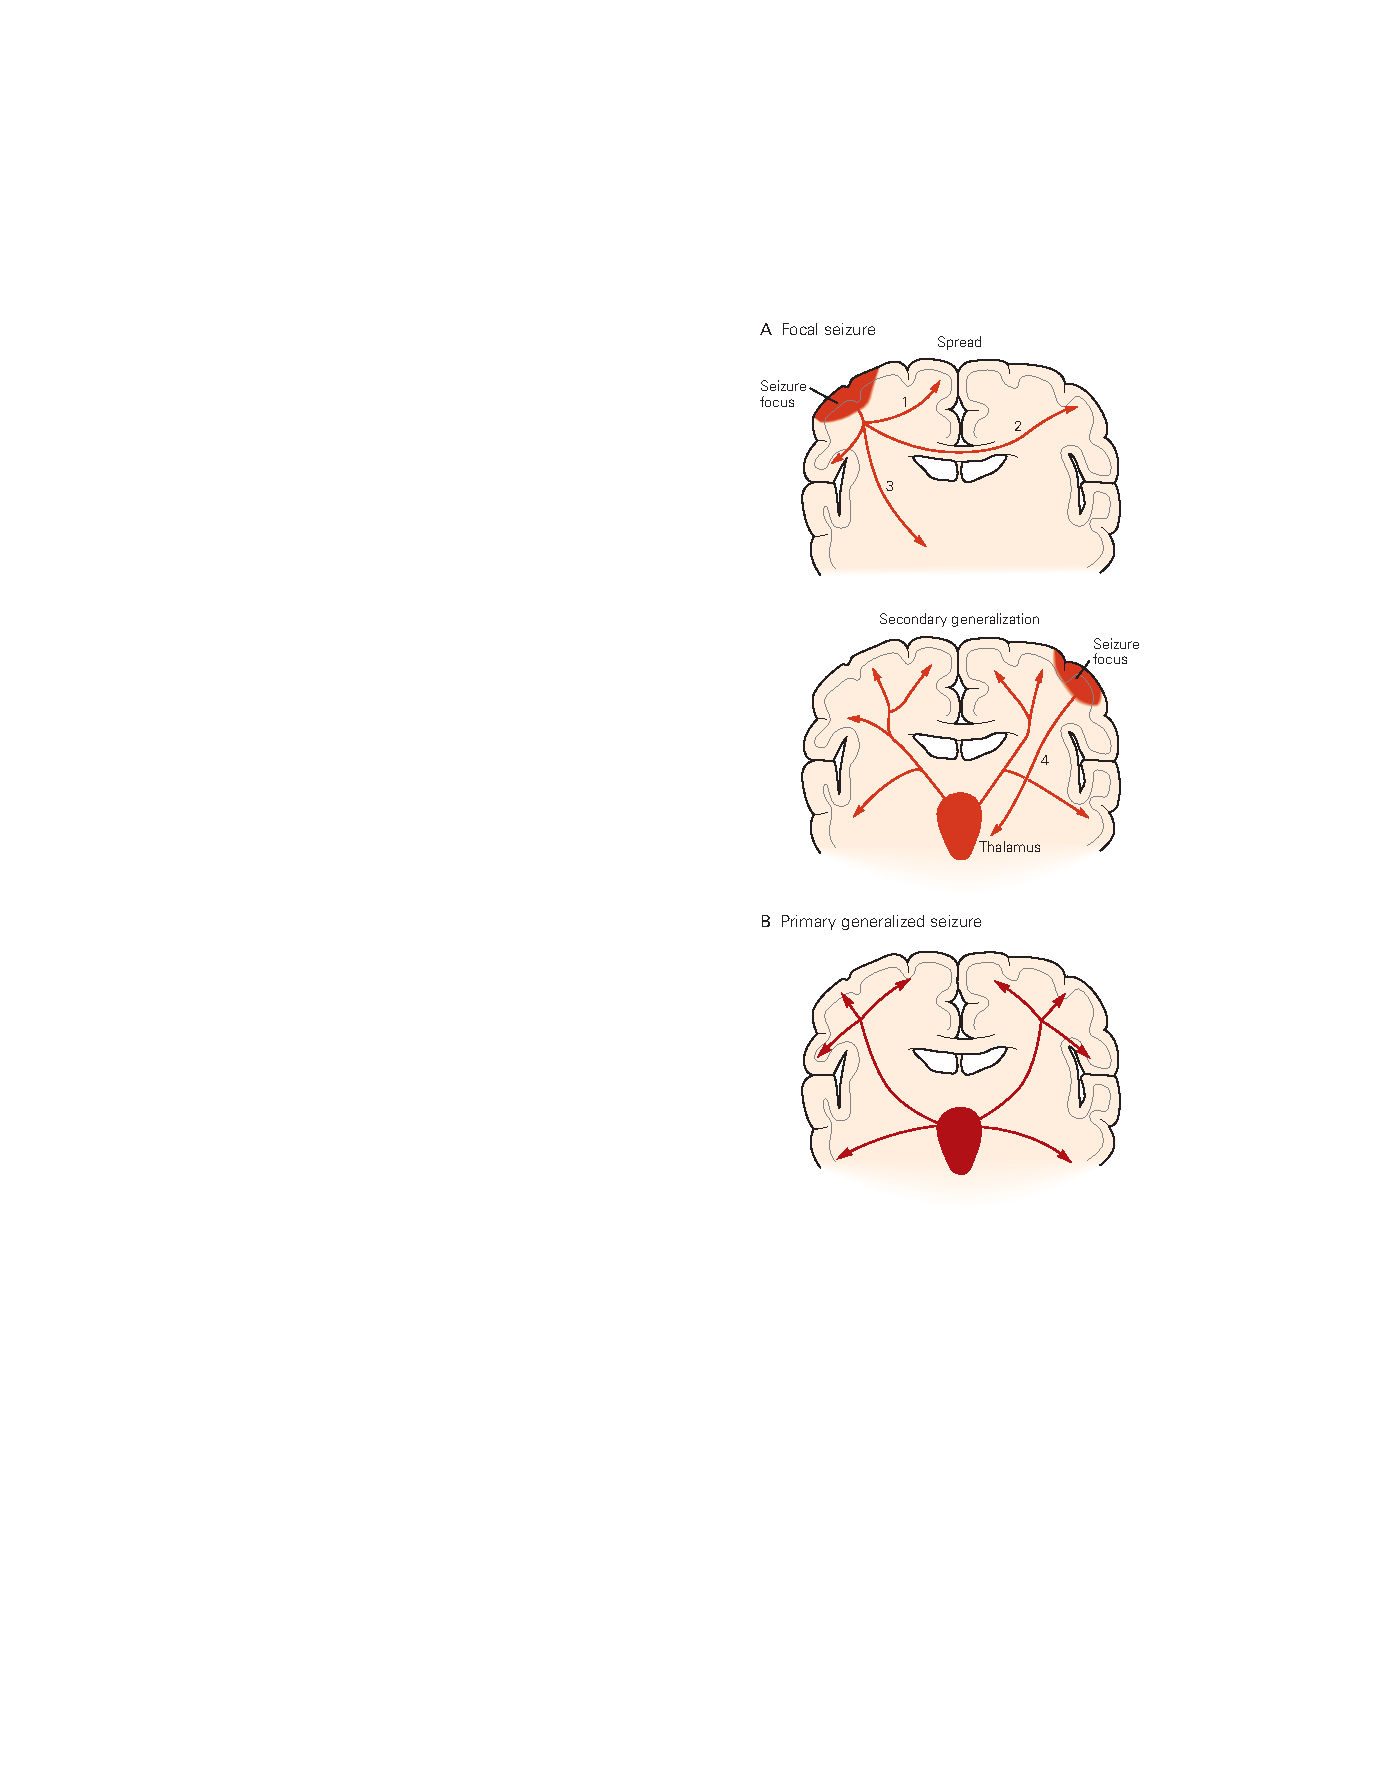
\includegraphics[width=0.4\linewidth]{chap58/fig_58_10}
	\caption{局灶性和全身性发作通过多种途径传播。 (经许可改编自 Lothman 1993b。)A. 局灶性癫痫发作可以通过大脑半球内纤维 (1) 从病灶局部扩散,并更远地扩散至同伦对侧皮层 (2) 和皮质下中心 (3)。 局灶性癫痫发作的继发性泛化通过投射到丘脑扩散到皮质下中心 (4)。广泛的丘脑皮质互连随后有助于两个半球的快速激活。B. 在全身性癫痫发作中,例如典型的失神发作,丘脑和皮层之间的相互联系是癫痫发作传播的主要途径。}
	\label{fig:58_10}
\end{figure}


一个有趣的悬而未决的问题是什么可以终止癫痫发作。
值得注意的是,几乎没有明确定义自我限制返回发作间期状态的机制。
此时的一个明确结论是终止不是由于细胞代谢耗尽,因为在严重的条件下,临床癫痫发作可能会持续数小时(见下文)。
在继发全身性局灶性癫痫发作的最初 30 秒左右,受累区域的神经元会经历长时间的去极化并持续放电(由于通常在阵发性去极化偏移之后发生的后超极化消失)。
随着癫痫发作的发展,神经元开始复极化并且后超极化再次出现。
去极化和复极化的周期对应于癫痫发作的阵挛期(图 ~\ref{fig:58_7}A)。


癫痫发作后通常会出现一段时间的电活动减少,即发作后期,可能伴有意识模糊、嗜睡甚至局灶性神经功能缺损的症状,例如偏瘫(Todd 麻痹)。
一旦其他大脑区域恢复正常功能,当一个大脑区域或功能长期抑制时,发作后期的神经系统检查可以导致对发作焦点轨迹的洞察。



\section{全身性癫痫发作是由丘脑皮质回路驱动的}

与典型的局灶性癫痫发作不同,全身性癫痫发作会同时突然破坏两个大脑半球的正常大脑活动。
全身性发作及其相关癫痫的表现和病因各不相同。
尽管全身性发作的细胞机制与局灶性发作或继发性全身性发作在许多有趣的方面有所不同,但全身性发作很难在临床上或通过脑电图与迅速泛化的局灶性发作区分开来。


研究最多的全身性发作类型是典型的失神发作 (petit mal),其特征性 EEG 模式(图~\ref{fig:58_11}A 中的 3 Hz 棘波模式)于 1933 年首次被 Hans Berger 识别。
F. A. Gibbs 认识到这种 EEG 模式与典型的失神发作之间的关系(他恰当地将这种模式描述为“飞镖和圆顶”),并将该机制归因于全身性皮质紊乱。
典型失神发作的独特临床特征与 EEG 活动有明显的相关性。


\begin{figure}[htbp]
	\centering
	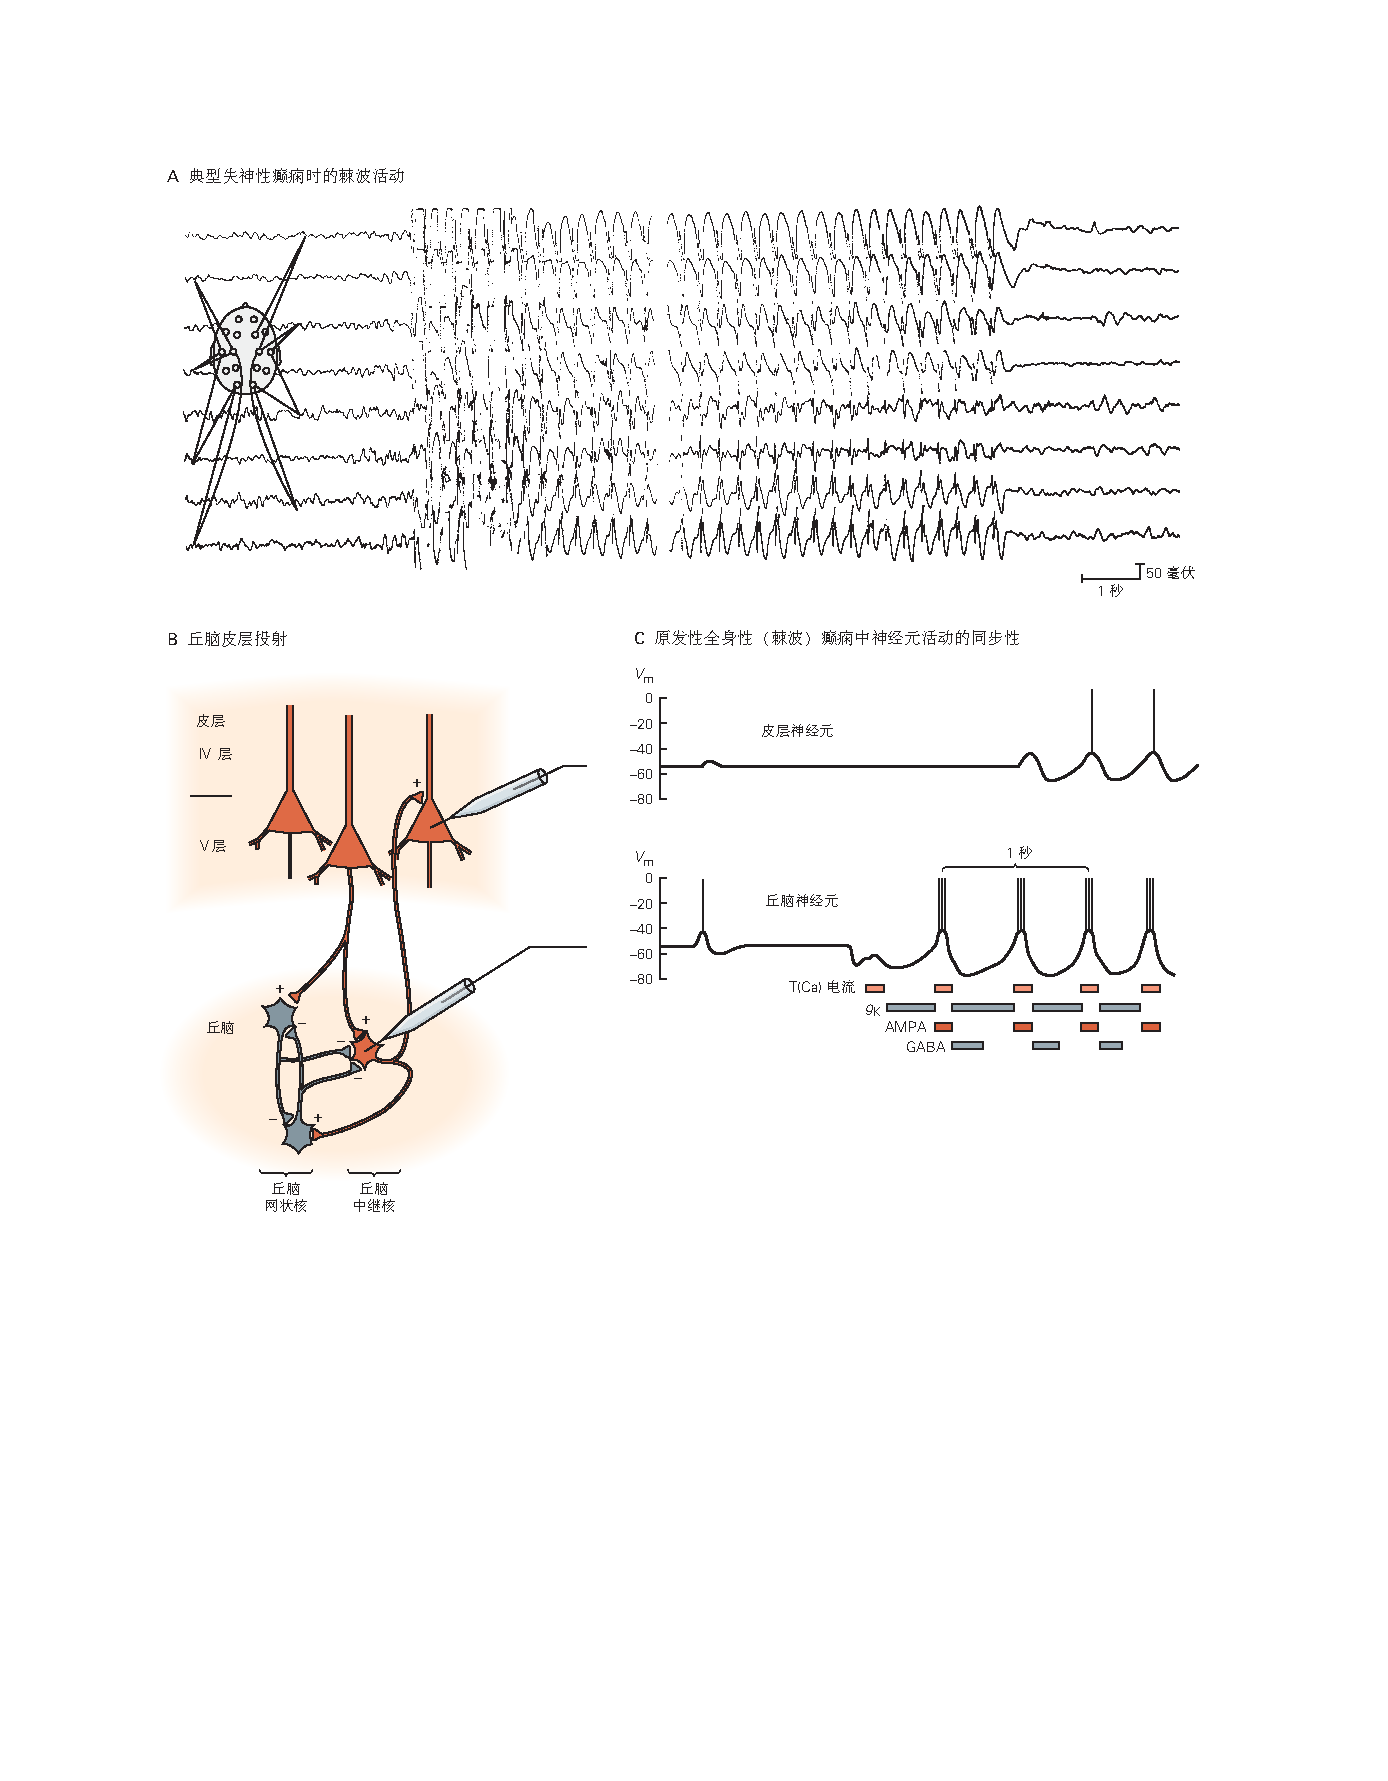
\includegraphics[width=0.9\linewidth]{chap58/fig_58_11}
	\caption{全身性发作具有独特的脑电图 (EEG) 和单神经元模式。A. 一名患有典型失神发作(小发作)的 12 岁患者的脑电图显示,同步尖峰突然出现,频率为每秒 3 次,波活动持续约 14 秒。癫痫发作在临床上表现为凝视,偶尔眨眼。与局灶性癫痫发作不同,癫痫发作前没有活动的积累,癫痫发作后电活动突然恢复到正常背景水平。迹线的不连续性是由于删除了 3 秒的记录周期。 (经许可转载自 Lothman 和 Collins 1990。)B. 参与睡眠纺锤波生成的丘脑皮质连接(第 ~\ref{chap:chap44}~章)被认为对于全身性癫痫发作的生成至关重要。皮层中的锥体细胞通过兴奋性突触与丘脑中继神经元相互连接。网状丘脑核中的 GABA 能抑制性中间神经元被皮质中的锥体细胞和丘脑中继神经元兴奋,并抑制丘脑中继细胞。中间神经元也相互连接。 C. 皮层和丘脑神经元的神经元活动在全身发作期间变得同步。去极化取决于 α-氨基-3-羟基-5-甲基-4-异恶唑丙酸 (AMPA) 型谷氨酸受体通道和 T 型电压门控 Ca2+ 通道中的电导。复极化是由于 γ-氨基丁酸 (GABA) 介导的抑制以及电压和钙依赖性 K+ 电导 (gK)。 (经许可改编自 Lothman 1993a。)}
	\label{fig:58_11}
\end{figure}


典型的失神发作突然开始,持续 10 到 30 秒,并产生意识障碍,只有轻微的运动表现,如眨眼或咂嘴。
与继发全身性发作的局灶性发作不同,全身性发作之前没有先兆,也没有发作后症状。
尖波脑电图模式可以突然并同时在所有大脑区域看到,并且紧接在正常背景活动之前和之后。
非常短暂(1-5 秒)的 3 赫兹脑电图活动没有明显的临床症状在失神发作患者中很常见,但如果频繁,它们会影响他们进行正常活动的能力,例如学校表现。


与 Gibbs 的弥漫性皮层过度兴奋假说相反,Penfield 和 Jasper 指出,典型失神发作中的脑电图类似于睡眠中的节律性脑电图活动,即所谓的睡眠纺锤波(第 ~\ref{chap:chap44}~章)。
他们提出了一个“中脑”假说,其中泛化归因于上脑干或丘脑中神经元聚集体的节律性活动(起搏),这些神经元聚集体扩散到皮质。


对全面性发作动物模型的研究和对全面性癫痫遗传学的研究表明,这两个假设的要素都是正确的。
在猫中,肠胃外注射青霉素(一种弱的 GABAA 拮抗剂)会产生与双侧同步慢波脑电图模式相关的行为反应迟钝(全身性青霉素癫痫)。
在这种癫痫发作期间,丘脑和皮层细胞通过相同的相互丘脑皮质连接变得同步,这些连接在慢波睡眠期间有助于正常的睡眠纺锤波。


这种癫痫发作在理论上可以代表大脑皮层中弥漫性过度兴奋的一种形式。
来自单个皮层神经元的记录显示在去极化爆发期间放电速率增加,这反过来产生强大的 GABA 能抑制反馈,在每次爆发后使细胞超极化约 200 毫秒(图~\ref{fig:58_11}C)。
这种抑制后的去极化与局灶性癫痫发作中的阵发性去极化转变根本不同,因为保留了 GABA 能抑制。
在典型的失神发作中,爆发的总和活动产生尖峰,而总抑制产生尖峰波 EEG 模式的波。


促进这种普遍和同步活动的细胞和网络的特性是什么?
早期的线索来自对丘脑中继神经元内在爆发的研究。
Henrik Jahnsen 和 Rodolfo Llinas 发现这些神经元强烈表达 T 型电压门控 Ca2+ 通道,该通道在静息膜电位下失活,但在细胞超极化时可用于激活(第 ~\ref{chap:chap10}~章)。
随后的去极化会暂时打开 Ca2+ 通道(因此得名 T 型),Ca2+ 流入会产生低阈值的 Ca2+ 尖峰。
与 T 型通道导致失神发作的假设一致,某些阻断失神发作的抗惊厥药,如乙琥胺 (Zarontin) 和丙戊酸 (Depakote),也会阻断 T 型通道。
T 型通道由三个相关基因 (Cav3.1–Cav3.3) 编码,其中 Cav3.1 是丘脑中的主要类型。


丘脑的回路似乎非常适合全身性癫痫发作的产生。
睡眠纺锤波期间丘脑神经元活动的模式表明丘脑中继神经元与丘脑网状核和膝周核中的 GABA 能中间神经元之间存在相互作用(图~\ref{fig:58_11}B)。
David McCormick 及其同事对丘脑切片的研究表明,中间神经元使中继神经元超极化,从而消除了 T 型 Ca2+ 通道的失活。
这一行动导致振荡反应:
在每个 IPSP 之后,T 型 Ca2+ 通道产生的动作电位反弹爆发会刺激 GABA 能中间神经元,导致另一轮中继神经元反弹放电。
中继神经元还激发皮层神经元,在 EEG 中表现为“纺锤体”。
T 型 Ca2+ 通道和 GABAB 受体通道在这种活动的产生中起着重要作用,类似于人类失神发作(第~\ref{chap:chap44}~章)。


电压门控 Ca2+ 通道的突变产生了几种全身性癫痫小鼠模型,包括所谓的蹒跚小鼠,它在参与神经递质释放的 P/Q 型钙通道中发生突变。
Jeffrey Noebels 和他的同事对这些突变体的研究表明,这些动物在进入青春期时会出现全身性癫痫发作。
这些动物的脑电图显示阵发性棘波放电和癫痫发作,其特征是行为停止和乙琥胺阻滞,类似于儿童的典型失神发作。
这些小鼠的丘脑神经元具有升高的 T 型 Ca2+ 通道,有利于反弹爆发。
现在已经在小鼠中描述了这种表型的 20 多种不同基因的突变。
值得注意的是,许多编码参与突触前递质释放的离子通道亚基或蛋白质。



\section{定位发作病灶对癫痫的手术治疗至关重要}

Wilder Penfield 于 1950 年代初在蒙特利尔进行的开创性研究使人们认识到,切除某些海马起源的局灶性癫痫发作患者的颞叶可以减少癫痫发作的次数,甚至可以治愈癫痫。
随着此类患者的手术治疗变得越来越普遍,很明显手术结果与切除的充分性直接相关。
因此,在局灶性癫痫发作的情况下精确定位癫痫病灶至关重要。
癫痫病灶的电映射最初依赖于表面脑电图,我们已经看到它偏向于紧邻颅骨的皮层中的特定神经元组。
然而,常规医学治疗难以治疗的癫痫发作通常始于深层结构,在癫痫发作开始时表面脑电图显示很少或没有异常。
因此,表面脑电图在确定癫痫病灶的位置方面有些局限。



磁共振成像的发展显着改善了癫痫病灶的无创解剖映射。
这种技术现在是评估涉及颞叶的癫痫的常规方法,但也显示出越来越有希望识别其他位置的癫痫病灶。
通过核磁共振成像对癫痫病灶进行解剖定位的科学基础是观察到大多数伴有意识障碍的顽固性局灶性癫痫发作患者的海马结构内侧部分出现萎缩和细胞丢失。
海马体内的神经元急剧减少(内侧颞叶硬化),存活细胞的树突形态发生变化,一些轴突侧生出芽。
现代核磁共振成像机器的解剖分辨率允许对癫痫患者的海马体大小进行无创、定量评估。
大脑一侧或另一侧海马体体积的减少通常与使用植入深度电极的功能标准确定的海马体癫痫病灶定位密切相关。


典型的颞叶内侧癫痫患者有单侧疾病,导致一侧海马体萎缩,这可能与侧脑室颞角的明显扩张有关。
方框~\ref{box:58_3}说明了这种情况。
然而,在许多患者中,使用解剖核磁共振成像无法检测到异常;
因此,非解剖学(功能)成像技术 (\textit{功能性磁共振成像}) 也被使用(第~\ref{chap:chap6}~章)。


\begin{proposition}[神经解剖学导航术语] \label{box:58_3}
	
	\quad \quad 一名27岁的女性从19岁开始出现反应性下降的症状。
	起初,她会瞪大眼睛,在剧集中显得很困惑。
	后来,她形成了一种由恐惧感组成的气场。
	在这种恐惧之后,意识发生了变化,瞪大了眼睛,左臂收紧,尖叫持续了14到20秒(图58-12)。
	
	\quad \quad 这些症状被诊断为复杂的部分性癫痫发作。
	尽管使用了几种抗癫痫药物,癫痫发作每周仍会发生几次。
	由于经常癫痫发作,她无法工作或开车。
	她在6个月大时就有脑膜炎病史,在整个童年时期,她都经历过短暂的认知改变,被描述为“就像有人扔了一个开关”。
	
	\quad \quad 根据图58–13和58–14中总结的评估,进行了右侧杏仁核-海马切除术。
	患者在手术后没有癫痫发作,并返回全职工作岗位。
	
\end{proposition}


功能性神经影像学利用发作期和发作间期发作病灶中发生的脑代谢和血流变化。
与癫痫发作相关的电活动对脑组织提出了大量的代谢需求。
在局灶性癫痫发作期间,葡萄糖和氧气的利用率大约增加了三倍。
在癫痫发作之间,癫痫病灶通常表现为新陈代谢下降。
尽管代谢需求增加,但大脑能够在局灶性癫痫发作期间维持正常的三磷酸腺苷 (ATP) 水平。
另一方面,全身性运动发作期间呼吸的短暂中断会导致血液中的氧气水平降低。
这导致 ATP 浓度下降和厌氧代谢增加,如乳酸水平升高所示。
这种氧债在发作后期会迅速得到补充,单次全身性癫痫发作不会对脑组织造成永久性损伤。


起源于内侧颞叶的局灶性发作患者的正电子发射断层扫描 (PET) 扫描经常显示发作间期代谢减退,代谢变化延伸至外侧颞叶、同侧丘脑、基底神经节和额叶皮层。
使用不可水解葡萄糖类似物的 PET 扫描特别有助于识别 核磁共振成像扫描正常的患者和一些儿童早期癫痫患者的发作灶。
不幸的是,由于不明原因,PET 在定位额叶等颞外区域的癫痫病灶方面不太可靠。
另一个限制是 PET 扫描的费用和同位素的半衰期短(需要附近的回旋加速器)。
PET 扫描还可用于寻找与癫痫发作活动相关的神经递质受体结合和运输的功能变化。


一种测量脑血流量的相关技术,即单光子发射计算机断层扫描 (SPECT),已比 PET 更频繁地使用。
SPECT没有PET的分辨率,但可以在很多大医院的核医学科进行。
在癫痫发作时注射放射性同位素和 SPECT 成像(发作期 SPECT)揭示了癫痫病灶和周围组织代谢亢进随后代谢减退的模式。
脑磁图和功能性核磁共振成像在绘制癫痫病灶方面也具有更多优势。


通过严格选择癫痫手术患者,颞叶明确发作病灶的癫痫治愈率可接近 80\%。
具有复杂因素(例如,多个病灶)的患者成功率较低。
然而,即使在这些患者中,癫痫发作的次数和严重程度通常也会降低。
已经“治愈”癫痫发作的患者可能仍会遇到记忆力减退等认知问题和社会问题,例如适应更独立的生活和有限的就业机会。
这些因素强调了尽早接受治疗的必要性。



\section{长时间癫痫发作会导致脑损伤}

\subsection{反复惊厥发作是一种医疗急症}

如上所述,脑组织可以代偿局灶性癫痫发作的代谢应激或单次全身性强直阵挛发作期间氧气输送的短暂减少。
在全身性癫痫发作中,下丘脑的刺激会导致交感神经系统“应激”反应的大量激活。
增加的全身血压和血糖最初补偿增加的代谢需求,但这些稳态机制在长时间癫痫发作期间失效。
由此产生的全身代谢紊乱,包括缺氧、低血压、低血糖和酸血症,会导致大脑中高能磷酸盐(ATP 和磷酸肌酸)减少,从而对脑组织造成破坏。


全身并发症如心律失常、肺水肿、体温过高和肌肉衰竭也可能发生。
反复全身性癫痫发作而癫痫发作之间未恢复完全意识的情况称为癫痫持续状态,是一种真正的医疗急症。
这种情况需要积极的癫痫发作管理和一般医疗支持,因为 30 分钟或更长时间的连续痉挛性癫痫发作会导致脑损伤甚至死亡。
癫痫持续状态可能涉及非惊厥性癫痫发作,其代谢后果要轻得多。


除了癫痫持续状态的危险外,癫痫发作控制不佳的患者也有猝死的风险(癫痫突然意外死亡 [SUDEP]),这是癫痫发作未控制患者死亡的主要原因。
SUDEP 的潜在机制尚不完全清楚,但 Richard Bagnall 及其同事以及其他人最近的研究表明,SUDEP 病例在涉及心律失常和癫痫的基因中具有临床相关突变。
这些数据支持 SUDEP 与心律失常或参与呼吸控制的脑干回路中断之间的关联。
这个话题恰如其分地成为当前激烈调查的焦点。



\subsection{兴奋性毒性是癫痫发作相关脑损伤的基础}

反复发作可独立于心肺或全身代谢变化而损害大脑,这表明大脑中的局部因素可导致神经元死亡。
未成熟的大脑似乎特别容易受到这种损害,这可能是因为发育中的大脑神经元之间的电紧张耦合更强,未成熟的神经胶质细胞对钾的缓冲效果较差,以及葡萄糖跨血脑屏障的转运减少。


1880 年,威廉·索默 (Wilhelm Sommer) 首次注意到海马体对此类损伤的脆弱性,其中 CA1 和 CA3 区域的锥体神经元优先丢失。
通过对海马体的传入神经进行电刺激或通过注射兴奋性氨基酸类似物(如红藻氨酸),已在实验动物中复制了这种模式。
有趣的是,红藻氨酸会在注射部位以及源自注射部位的传入神经终止部位造成局部损伤。


这些观察结果表明,在过度刺激(例如癫痫发作)期间释放兴奋性递质谷氨酸盐本身会导致神经元损伤,这种情况称为兴奋性毒性。
因为在癫痫持续状态期间很难检测到细胞外谷氨酸的增加,所以兴奋性毒性似乎更多地是由谷氨酸受体的过度刺激引起的,而不是细胞外谷氨酸的强直性增加。
急性兴奋性毒性的组织学表现包括细胞体和树突的大量肿胀、谷氨酸受体和兴奋性突触的主要位置。


尽管兴奋性毒性的细胞和分子机制仍未完全了解,但有几个特征是明确的。
谷氨酸受体的过度激活会导致细胞内 Ca2+ 过度增加,从而激活涉及钙依赖性酶(如磷酸酶、蛋白酶和脂肪酶)的自毁性细胞级联反应。
脂质过氧化还会导致自由基的产生,从而破坏重要的细胞蛋白质并导致细胞死亡。
线粒体在 Ca2+ 稳态和自由基控制中的作用也可能很重要。 细胞死亡的模式最初被认为反映了由于关键细胞蛋白的自溶而导致的坏死。
然而,也可能涉及程序性细胞死亡(细胞凋亡)的特征“死亡基因”的激活。


与癫痫发作相关的脑损伤或兴奋性中毒可能特定于特定大脑区域的某些类型的细胞,这可能是由于保护因素,例如某些细胞中的钙结合蛋白和敏化因素,例如钙渗透性谷氨酸受体的表达 其他细胞。
例如,由 AMPA 型谷氨酸受体过度激活引起的体外兴奋性毒性优先影响表达具有高 Ca2+ 渗透性的 AMPA 型受体的中间神经元,这为它们的选择性脆弱性提供了可能的机制。


几起“遗忘性”贝类中毒事件为谷氨酸受体过度激活的后果提供了一个生动的例子。
软骨藻酸是一种不存在于大脑中的谷氨酸类似物,是某些海藻种类的天然产物,它们在适当的海洋条件下繁盛。
贝类等滤食性动物可浓缩软骨藻酸。
偶尔摄入受 domoic 污染的贝类会导致神经系统损伤的爆发,包括严重的癫痫发作和记忆力减退(健忘症)。
对损伤最敏感的区域是海马体,这进一步支持了兴奋性毒性假说和海马体在学习和记忆中的关键作用。



\section{导致癫痫发展的因素知之甚少}

单次发作不能保证诊断为癫痫。
正常人在药物摄入或极度睡眠剥夺后等情有可原的情况下可能会发作。
临床医生寻找此类患者癫痫发作的可能原因,但通常不会在单次癫痫发作后开始使用抗惊厥药进行治疗。
不幸的是,我们对导致癫痫易感性的因素的了解仍然很初级。
然而,随着动物模型实验诱变和患者临床神经遗传学(包括全外显子组测序)的出现,这方面的进展正在迅速增加。


长期以来,某些形式的癫痫一直被认为部分是由遗传倾向引起的。
例如,患有热性惊厥的婴儿通常有类似惊厥的家族史。
遗传学在癫痫中的作用得到了人类家族性癫痫综合征以及易发癫痫动物模型的支持,这些动物模型具有诸如 Papio papio(具有光敏性癫痫发作的狒狒),听觉小鼠(其中大声诱发癫痫发作)和 自发的单位点突变,例如卷线鼠和蹒跚鼠(名称暗指这些动物小脑突变的临床表现)。
即使有遗传倾向或结构性损伤,癫痫表型的演变也常常涉及大脑结构和功能的适应不良变化。



\subsection{离子通道突变是癫痫的遗传原因之一}

最近的研究提供了大量关于癫痫分子遗传学的新信息。 目前,已有 120 多个基因与癫痫表型相关;
其中大约一半是在人类身上发现的,其他是在动物身上发现的,主要是老鼠。
受影响的蛋白质包括离子通道亚基、参与突触传递的蛋白质,如转运蛋白、囊泡蛋白、突触受体和参与 Ca2+ 信号传导的分子。
例如,蹒跚突变小鼠的癫痫发作是由于编码 P/Q 型电压门控 Ca2+ 通道的 CaV2.1 或 α1A 亚基的基因发生自发突变。
考虑到癫痫发作对突触传递和神经元兴奋性的依赖性,这类蛋白质的突变可能会导致癫痫症,这也许并不出人意料。


一些与小鼠癫痫相关的其他基因更令人惊讶,例如着丝粒 BP-B 的基因,一种\textit{脱氧核糖核酸}结合蛋白,以及在慢波癫痫小鼠中受到影响的钠/氢交换基因。
各种各样的人类基因会导致神经系统疾病,癫痫只是其中的一种表现形式。
例如,雷特综合征是一种与智力障碍、自闭症和癫痫发作相关的疾病,是由基因转录调节因子 MECP2(甲基-CpG 结合蛋白-2)的突变引起的。
虽然确切的联系尚不清楚,但很明显许多不同基因的突变可能导致癫痫。


在大多数情况下,人类的遗传性癫痫综合征具有复杂而不是简单的(孟德尔)遗传模式,这表明涉及许多而不是单个基因。
尽管如此,在对癫痫家族的研究中已经发现了一些单基因癫痫。
Ortrud Steinlein 及其同事在 1995 年报告说,烟碱型乙酰胆碱受体通道的 α4 亚基突变是常染色体显性夜间额叶癫痫 (ADNFLE) 的原因,这是人类癫痫常染色体基因缺陷的第一个例子。
随后,其他电压和配体门控通道蛋白已被确定为癫痫的关键基因。
离子通道基因突变(通道病)是已知单基因癫痫的主要原因(图 58-15)。
通过针对从头突变的临床外显子组分析,正在发现更多的基因。
K+ 通道的大量基因以及这些通道在平衡兴奋和抑制中的关键作用是扩大癫痫基因组的重要原因。


在电压门控通道中,突变主要涉及主要的成孔亚基,但也有调节亚基中引起癫痫的突变的例子。
在体外检查时,突变通道蛋白通常与质膜表面通道表达的减少(由于对膜的靶向减少或过早降解)或通道动力学改变有关。
很容易考虑离子通道门控的变化如何影响神经元的兴奋性及其在癫痫发作期间的同步。
然而,离子通道突变也可能影响神经元发育,从而通过对细胞迁移、网络形成或基因表达模式的次级作用发挥其致癫痫作用。


在癫痫基因研究的早期,人们普遍认为这些基因主要是全身性癫痫的基础,基于基因突变(例如,在离子通道中)预计会影响大多数神经元的想法。
然而,Steinlein 及其同事发现的第一个常染色体显性遗传性癫痫基因引起局灶性发作(额叶)癫痫,另一个引起起源于颞叶的癫痫发作,伴有听觉先兆。
回想起来,这并不令人惊讶,因为通道亚基很少在大脑中统一表达,并且一些大脑区域比其他区域更容易产生癫痫发作。


基因表达的时间也很重要。
例如,在 P/Q 型 Ca2+ 通道的成孔 CaV2.1 亚基中发生突变的蹒跚小鼠在出生后第三周开始出现棘波型癫痫发作,这可能是因为 N 型 Ca2+ 通道是早期的主要功能亚型 在发展中,而 P/Q 型 Ca2+ 通道在后期占主导地位。
一旦在发育过程中功能需要突变通道,神经表型就开始了。


此外,一种突变可以引起不同的癫痫表型,或者不同的突变基因可以引起相同的癫痫表型。
作为后者的一个例子,ADNFLE 综合征最初是作为烟碱 ACh 受体的 α4 亚基突变发现的,也可能由 α2 亚基突变引起。
但并非所有携带这种常染色体显性突变的家庭成员都患有癫痫,这表明即使在这种形式的单基因癫痫中,其他基因和非遗传因素也会影响表型。
GEFS+ 综合征(全身性癫痫伴热性惊厥)是这种异质性的一个很好的例子。 这是一种儿童综合症,可能涉及不同家庭成员的不同癫痫发作类型。
GEFS+ 见于具有三种不同 Na+ 通道亚基之一或两种 GABAA 受体之一的基因突变的家族。
全面性发作性癫痫的家族研究表明,癫痫发作类型可能在家族内遗传。
这些发现表明,即使是单基因癫痫也可能被其他基因、环境影响甚至突触中依赖于经验的变化所改变。


皮层发育改变可能是癫痫的常见原因。
核磁共振成像扫描分辨率的提高揭示了癫痫患者出乎意料的大量皮质畸形和异常皮质折叠的局部区域。
因此,干扰皮层或网络布线正常形成的突变是癫痫的候选基因。
这个想法得到了两个 X 连锁皮质畸形与癫痫表型映射的支持:家族性脑室周围异位和家族性皮质下带异位。
分别编码细丝蛋白 A 和双皮质素的导致这两种疾病的基因可能在神经元迁移中很重要。
小的局灶性皮质发育不良可作为癫痫病灶,引起部分和继发性全身性癫痫发作,而更广泛的皮层畸形可引起多种癫痫发作类型,并且通常与其他神经系统问题有关。


另一个 X 连锁基因,aristaless 相关同源框 (ARX),是细胞类型特异性转录因子改变迁移的一个例子,因为它仅在中间神经元前体中表达。
一个特别有启发性的例子是癫痫与结节性硬化症 (TSC) 的关联,TSC 是一种常染色体显性遗传病,由于缺乏功能性 Tsc1-Tsc2 复合物,导致哺乳动物雷帕霉素靶标 (mTOR) 复合物 1 过度活跃 ( mTORC1) 信号通路。
mTOR 抑制剂作为这些患者难治性癫痫治疗的早期临床试验一直很有希望。
这些例子为将癫痫综合征的潜在生物学与临床相关治疗联系起来提供了希望。


在临床外显子组测序和对导致神经网络不稳定的生物学途径的认识的推动下,癫痫基因组正在迅速扩大。
不幸的是,即使最近癫痫基因鉴定的激增,也无法解释绝大多数癫痫病例。
通过在线登记对大量患者进行鉴定可能会提供评估构成复杂遗传模式基础的易感基因所需的群体样本。



\subsection{获得性癫痫的起源是对损伤的适应不良反应}

癫痫通常发生在不连续的皮层损伤(例如头部穿透伤)之后。
这种损伤是癫痫病灶的病灶,在稍后的某个时间点导致癫痫发作。
这导致了这样的想法,即早期的侮辱会引发一系列渐进的生理或解剖学变化,从而导致慢性癫痫发作。
也就是说,损伤和复发性癫痫发作之间的特征性“沉默”间隔(通常为数月或数年)可能反映了进行性适应不良的分子和细胞变化,这些变化可能适合治疗操作。
尽管是一个有吸引力的假设,但尚未出现关于这一过程的统一图景。
最有希望的证据来自对从接受颞叶切除术的患者和边缘癫痫发作的啮齿动物模型中取出的组织的研究。


在一个实验模型中,过度兴奋是由边缘结构(如杏仁核或海马体)的反复刺激引起的。
最初的刺激之后是电反应(后放电),随着重复刺激,电反应变得更加广泛和延长,直到发生全面性癫痫发作。
这个过程称为点燃,可以由电刺激或化学刺激引起。
许多研究人员认为,点燃可能会导致人类癫痫的发展。


点燃被认为涉及海马结构中的突触变化,类似于学习和记忆中的重要变化(第~\ref{chap:chap53}~和 ~\ref{chap:chap54}~章)。
这些包括兴奋性的短期变化和持续的形态变化,包括成年神经元的产生、轴突萌芽和突触重组。
在长期颞叶癫痫患者的齿状回以及实验动物的点燃后观察到突触连接的重排。
除了轴突萌芽(图 58-16)外,变化还包括树突结构的改变、递质释放的控制,以及离子通道和泵的亚基化学计量的新表达和改变。


导致癫痫的长期变化也可能涉及特定的基因表达模式。
例如,原癌基因 c-fos 和其他直接早期基因以及生长因子可以被癫痫激活。
由于许多直接早期基因编码控制其他基因的转录因子,癫痫样活动产生的基因产物可能会通过改变细胞命运、轴突靶向、树突生长和突触形成等机制来引发有助于或抑制癫痫发展的变化。



\section{亮点}

1. 癫痫发作是哺乳动物大脑集体电行为最引人注目的例子之一。
部分性发作和全身性发作的独特临床模式可归因于皮质神经元明显不同的活动模式。


2. 对动物局灶性癫痫发作的研究揭示了一系列事件——从癫痫病灶中神经元的活动到癫痫样活动在整个皮层的同步和随后扩散。
GABAergic 环绕抑制的逐渐丧失对于这一进程的早期步骤至关重要。
相反,全身性癫痫发作被认为是由丘脑皮质回路的活动引起的,可能与所有皮质神经元的膜兴奋性的普遍异常相结合。


3. 脑电图 (EEG) 长期以来一直为大脑皮层的电活动提供一个窗口,无论是在正常的觉醒阶段还是在癫痫发作等异常活动期间。
脑电图可用于识别与癫痫发作相关的某些电活动模式,但它对癫痫发作的病理生理学提供的了解有限。
现在可以使用几种更强大和无创的方法来定位部分性发作的病灶。
这导致癫痫手术在选定的患者中得到广泛和成功的应用,特别是那些海马起病的复杂部分性癫痫发作的患者。
侵入性方法检测癫痫发作和预防癫痫发作的前景为改善癫痫发作控制提供了额外的希望。


4. 应用于癫痫发作和癫痫研究的遗传学、分子学和现代细胞生理学方法的日益强大也带来了新的希望,即了解正常大脑活动的这些破坏将为癫痫患者提供新的治疗选择,因为 以及对哺乳动物大脑功能的新见解。


5. 对从急性发作到癫痫发展的进一步神经生物学研究应该提供超越抗惊厥药或癫痫手术标准选择的替代治疗策略。

